\section{Optimum Linear Filtering}
\begin{itemize}
	\item Discrete Time
	\item Proper random processes
	\item Minimum mean square error (MMSE), Linear processing MMSE (LMMSE)
	\item Theory by N. Wiener (1948) and A. Kolmogorov (1941)
\end{itemize}
The design of a Wiener Filter requires a priori information about the statistics of the data to be processed. The filter is optimum only when the statistical characteristics of the input data match the priori information on which the design of the filter is based on. When this information is not known completely, however, it may not be possible to design the Wiener Filter or else the design may no loner be optimum.A straightforward approach that we may use in such situation is the "estimate and plug" procedure. This is a two-stage process, whereby the filter first "estimates" the statistical parameters of the relevant signals and then "plugs" the results so obtained into a non recursive formula for computing the filter parameters. For real-time operation, this procedure has the disadvantage of requiring excessively elaborate and costly hardware. \\
A wide variety of recursive algorithms have been developed in the literature for the operation of linear adaptive filters. In the final analysis, the choice of the algorithm is determined by one or more of the following factors: 
\begin{itemize}
	\item rate of convergence
	\item misadjustment
	\item tracking
	\item robustness
	\item computational requirements
\end{itemize}
\begin{figure}[htbp]
	\centering
		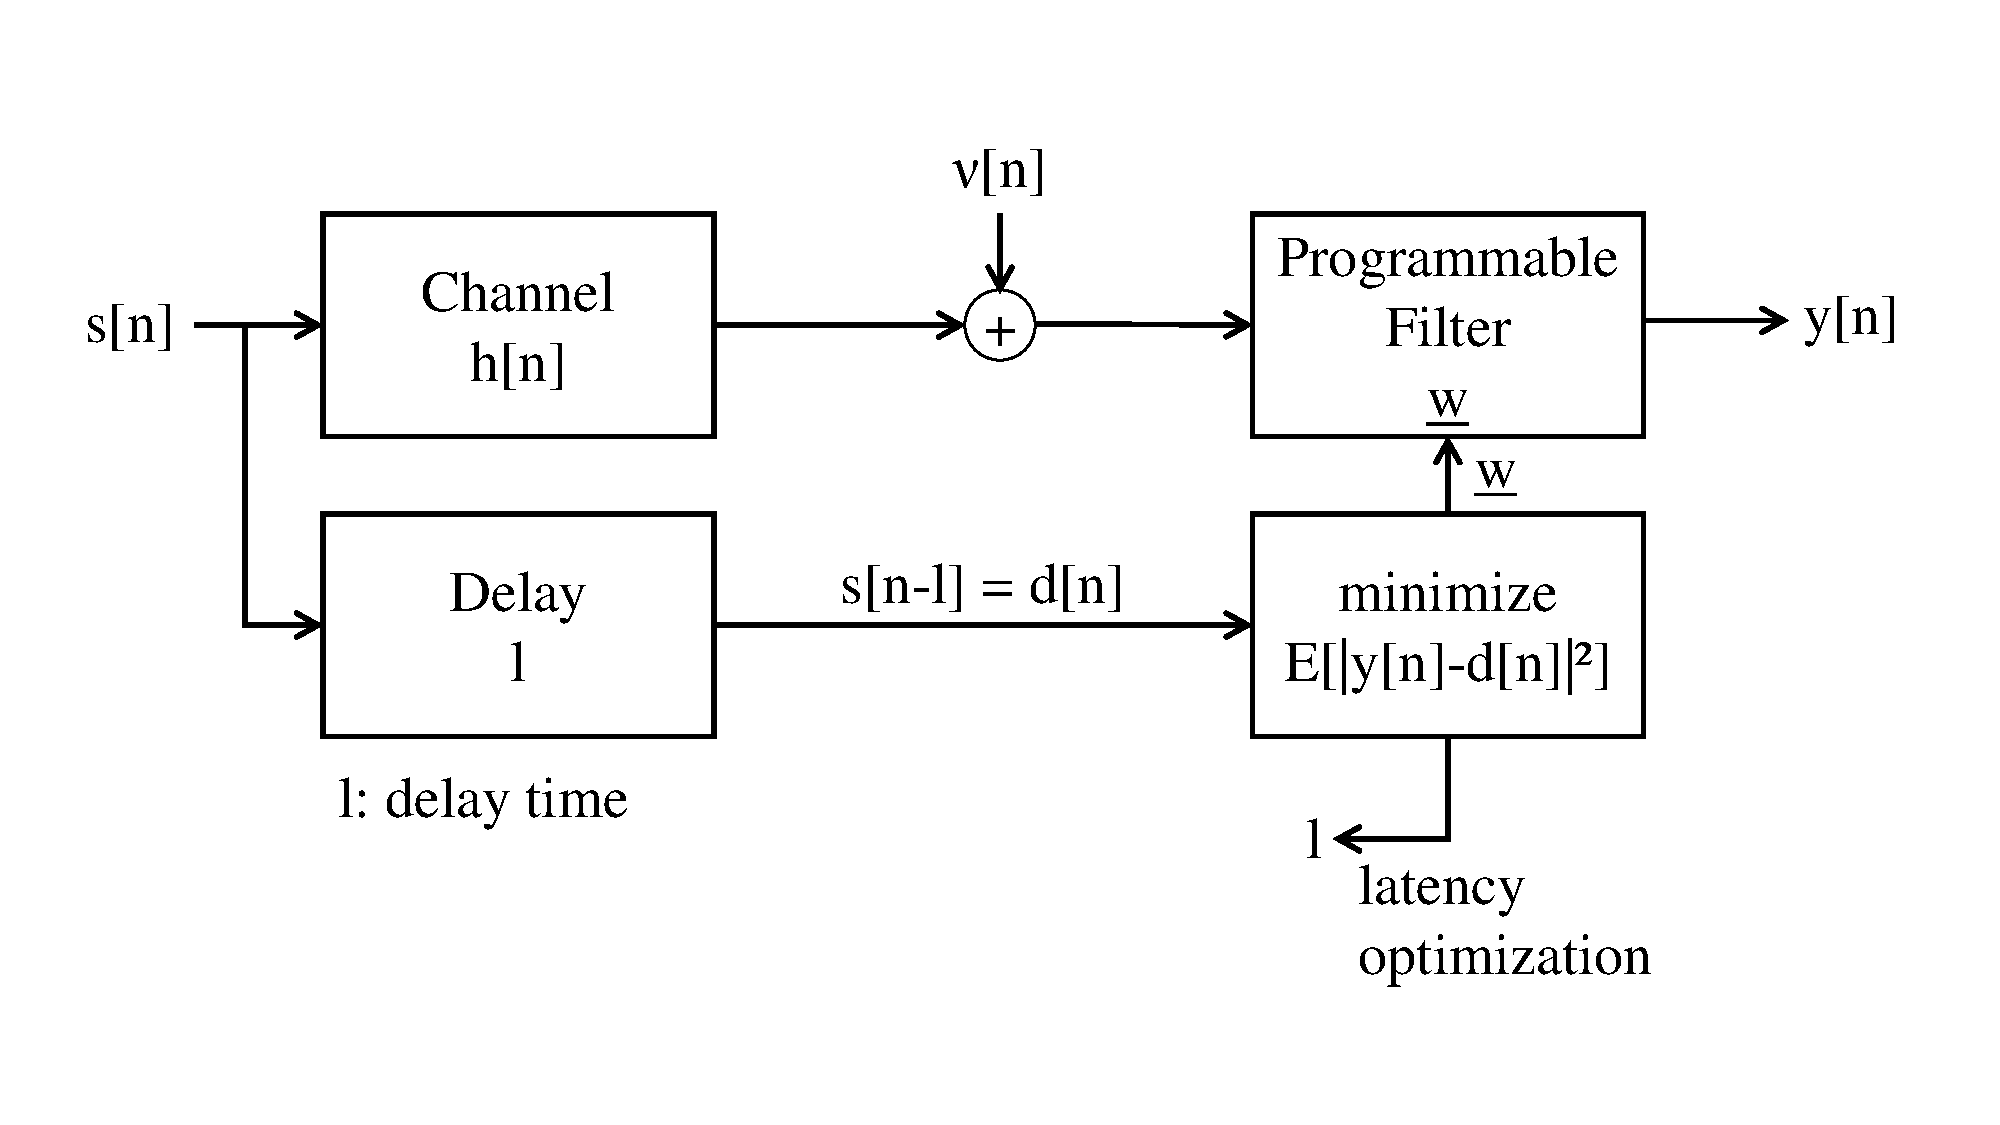
\includegraphics[width=0.80\textwidth, trim =1cm 2cm 1cm 2cm,clip ]{graphics/Optimum_filter_block_diagram.pdf}
	\caption{Basic block diagram of an Optimum Linear Filter}
	\label{fig:Optimum_filter_block_diagram}
\end{figure}

$x[n]=\sum\limits_{k=0}^{K} h[k] \cdot s[n-k]; \qquad K$: Channel memory ($0\leq K$)\\
$y[n]=\sum\limits_{k=0}^{M-1} w_k^* \cdot u[n-k]; \qquad M$: Number of filter coefficients (filter order) ($1\leq M$)\\

$\vec{x}[n] = \mat{x[n]\\ x[n-1]\\ \svdots \\ x[n-M+1]}; \qquad \vec{s}[n]= \mat{s[n]\\ s[n-1]\\ \svdots \\ s[n-N+1]}$\\

$\vec{x}[n] = \underbrace{\mat{h[0] & h[1] & h[2] & \shdots & h[K] & & 0 & \shdots & 0\\
													0 & h[0] & h[1] & h[2] & \shdots & h[K-1] & h[K] & 0 & \shdots & 0\\
													\ddots & \ddots & \ddots & \ddots & \ddots & \ddots & \ddots & \ddots & &\\
													0 & \shdots & 0 & h[0] & h[1] & h[2] & &\shdots & h[K-1] & h[K]}}_{\ma{H}} \cdot \vec{s}[n]$\\
\mybox{$\ma{H}\in \mathbb{C}^{M\times N}$\\$N=M+K \geq M $\\$\quad \Rightarrow$ wide Matrix} \\

$\vec{w} = \mat{w_0\\ w_1\\ \svdots \\w_{M-1}}; \qquad \vec{u}[n]=\vec{x}[n] + \vec{\nu}[n]; \qquad \vec{\nu}[n]$: Noise\\
$y[n] = \vec{w}^H \vec{u}[n] = \vec{w}^H(\vec{x}[n] + \vec{\nu}[n])$\\
\mybox{
$y[n] = \vec{w}^H (\ma{H}\vec{s}[n] + \vec{\nu}[n])$\\
with:\\
$y[n]$: Filter output\\
$\vec{w}^H$: Filter vector\\
$\ma{H}$: Channel matrix\\
$\vec{s}[n]$: Tx-signal vector\\
$\vec{\nu}[n]$: Noise vector
}
\subsection{Correlation between filter output and error in the optimum}
\begin{itemize}
	\item Error signal: $e[n]=d[n] - y[n]$
	\item Cost function: $J=E[|e[n]|^2]$
	\item Optimization: $\vec{w}_{opt} = \text{arg } \min\limits_{\vec{w}} J$
\end{itemize}

\begin{doublespace}

$J=E[e^*[n]\cdot e[n]] = E[(d^*[n] - y^*[n])(d[n]-\underbrace{y[n]}_{\vec{w}^H\vec{u}[n]})]$\\
$\frac{\partial J}{\partial \vec{w}^*} = E[e^*[n](-\vec{u}[n])] \stackrel{!}{=} 0$ (in the optimum)\\
$E[e^*[n]y[n]] = E[e^*[n]\vec{w}^H\vec{u}[n]] \underbrace{=}_{\vec{w}^H\ \text{deterministic}} \vec{w}^H\ E[e^*[n]\vec{u}[n]]=0$\\
in the optimum $\Leftrightarrow E[y[n]e^*[n]] = 0$ (Filter output is uncorrelated with error)\\
If you want to know, whether  a different filter is optimal or not, test if the error and the output are uncorrelated.

\subsection{Determine Optimal Filter Weight \texorpdfstring{$w_{opt}$}{w-opt}}
$J=E[(d^*[n] - y^*[n])(d[n]-y[n])] = \sigma_d^2 - \vec{w}^H\vec{p} - \vec{p}^H \vec{w} + \vec{w}^H \ma{R}\vec{w}$\\
$\sigma_d^2 = E[|d[n]|^2]$\\
$\vec{p} = E[\vec{u}[n]d^*[n]]; \qquad$ correlation vector\\
$\ma{R} = E[\vec{u}[n]\vec{u}^H[n]]; \qquad$ correlation matrix\\
Note: $\ma{R}\geq 0 \qquad$ usually $\ma{R}>0 \Rightarrow \ma{R}^{-1}$ exists\\$\qquad \ma{R}=\ma{R}^H$\\
$\frac{\partial J}{\partial \vec{w}^*}=-\vec{p} + \ma{R}\vec{w} \stackrel{!}{=} 0$\\
\mybox{
$\vec{w}_{opt}=\ma{R}^{-1}\vec{p}$}
$\vec{w}^H_{opt} = \vec{p}^H(\ma{R}^{-1})^H = \vec{p}^H(\ma{R}^{H})^{-1} = \vec{p}^H\ma{R}^{-1}$\\
$J\left.\right|_{\vec{w}=\vec{w}_{opt}}= \sigma_d^2 - \underbrace{\vec{p}^H\ma{R}^{-1}\vec{p}}_{=\vec{w}_{opt}\vec{p}} - \underbrace{\vec{p}^H\ma{R}^{-1}\vec{p} + \underbrace{\vec{p}^H\ma{R}^{-1}\ma{R}\ma{R}^{-1}\vec{p}}_{=\vec{p}^H\ma{R}^{-1}\vec{p}}}_{=0} = \sigma_d^2(1-\underbrace{\frac{\vec{p}^H\ma{R}^{-1}\vec{p}}{\sigma_d^2}}_{|\rho|^2}) \qquad 0\leq|\rho|^2\leq 1$
\end{doublespace}

\begin{figure}[htbp]
	\centering
		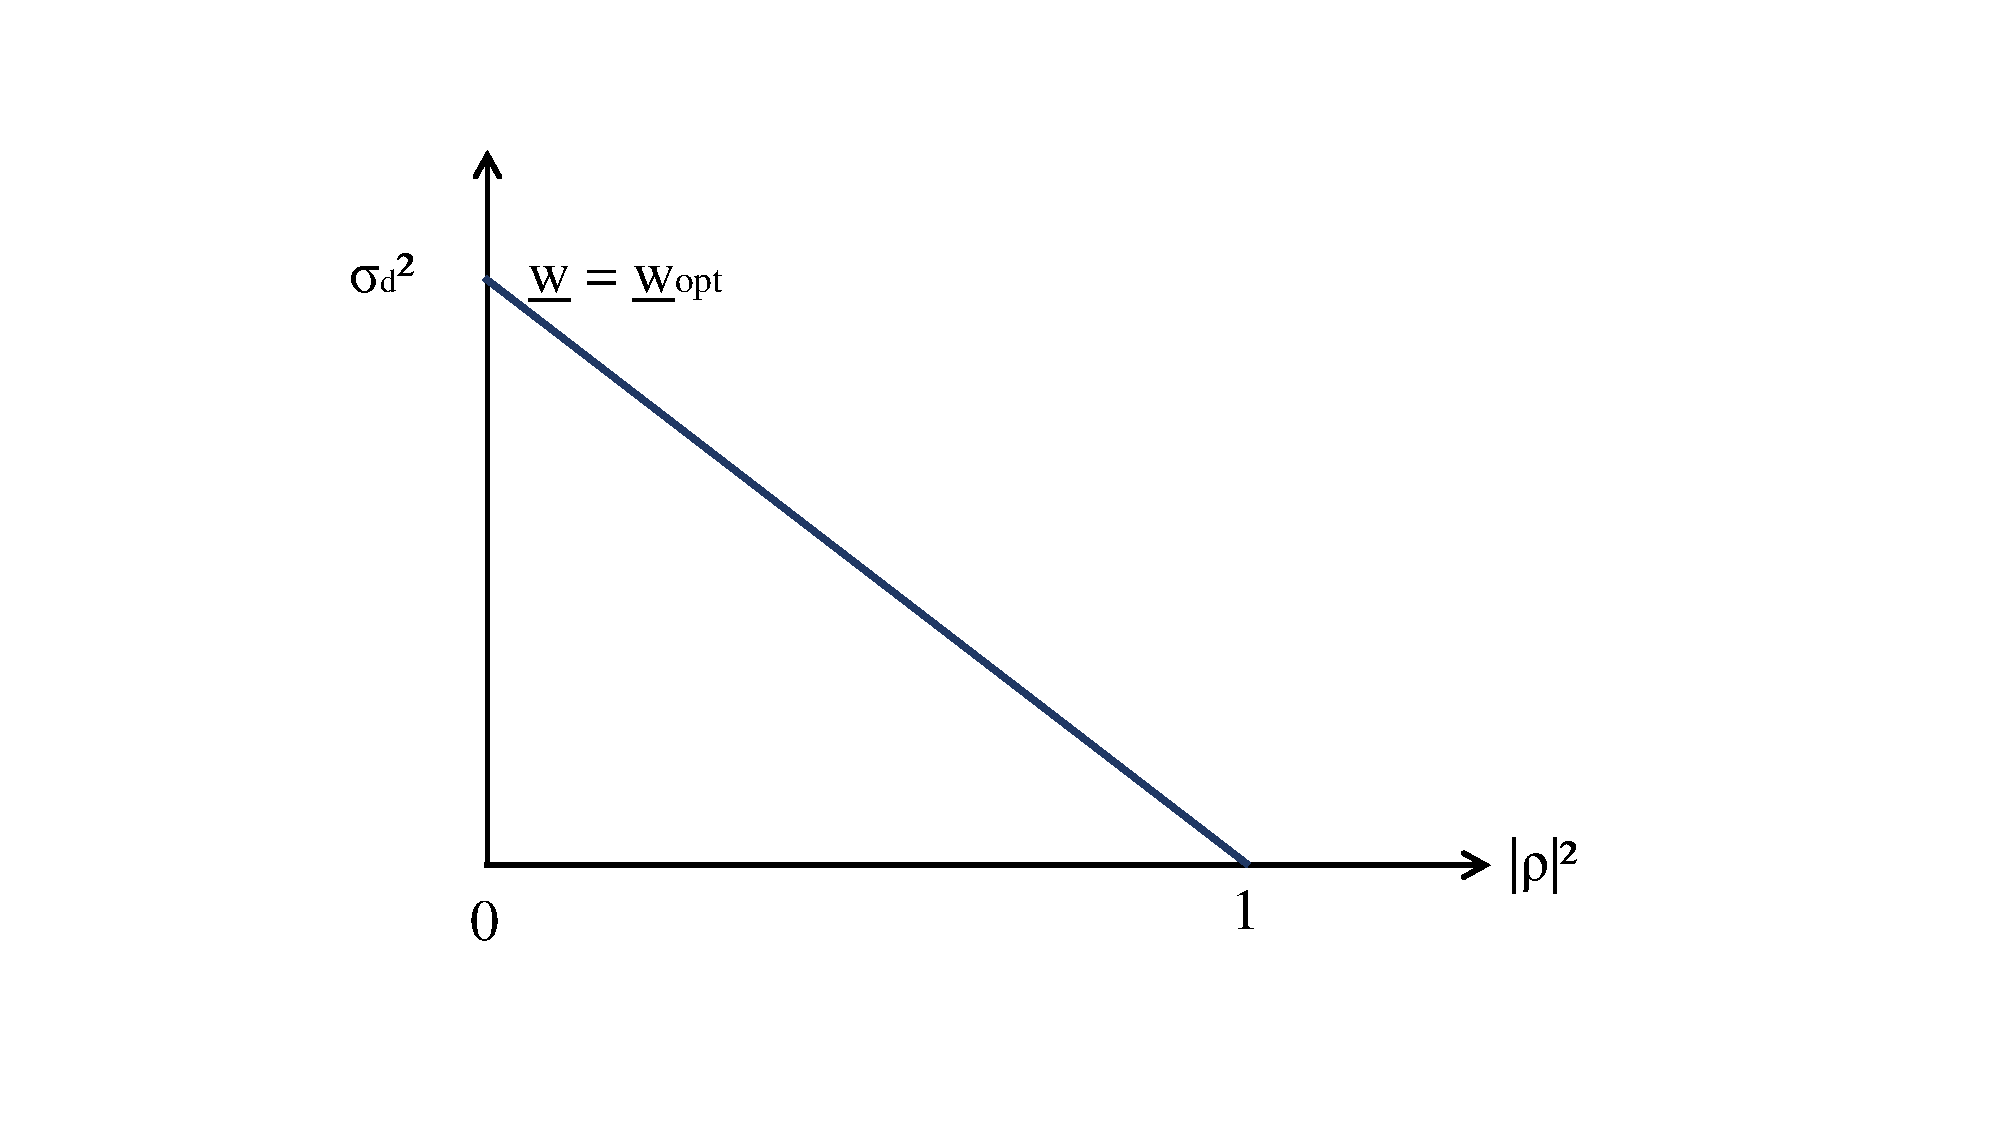
\includegraphics[trim =1cm 2cm 4cm 2cm, clip, width=0.80\textwidth]{graphics/diagram_rho_vs_sigma.pdf}
	\caption{Correlation betweem $\sigma_d^2$ and $|\rho|^2$}
	\label{fig:diagram_rho_vs_sigma}
\end{figure}

\begin{doublespace}
\begin{tabular}{ll}
$J$&$=\sigma_d^2 - \vec{w}^H\vec{p} - \vec{p}^H \vec{w} + \vec{w}^H \ma{R}\vec{w}$\\
&$=\sigma_d^2 - \vec{w}^H\ma{R}\underbrace{\ma{R}^{-1}\vec{p}}_{\vec{w}_{opt}} - \underbrace{\vec{p}^H \ma{R}^{-1}}
_{\vec{w}^H_{opt}} \ma{R} \vec{w} + \vec{w}^H \ma{R}\vec{w} + \vec{p}^H \underbrace{\ma{R}^{-1}\ma{R}\ma{R}^{-1}}_{\ma{R}^{-1}}\vec{p} - \vec{p}^H\ma{R}^{-1}\vec{p}$\\
&$=\sigma_d^2 - \vec{w}^H\ma{R}\vec{w}_{opt} - \vec{w}^H_{opt}\ma{R}\vec{w} + \vec{w}^H\ma{R}\vec{w} + \vec{w}^H_{opt}\ma{R}\vec{w}_{opt} - \vec{p}^H\ma{R}^{-1}\vec{p}$\\
&$=\underbrace{\sigma_d^2 - \vec{p}^H\ma{R}^{-1}\vec{p}}_{J_{min}} + \underbrace{(\vec{w}^H-\vec{w}^H_{opt})}_{\Delta\vec{w}^H}\ma{R} \underbrace{(\vec{w} - \vec{w}_{opt})}_{\Delta\vec{w}}$\\
&$=J_{\text{min}} + \underbrace{\Delta\vec{w}^H\ma{R}\Delta\vec{w}}_{>0 \quad \forall \Delta\vec{w}\neq 0 \quad \text{because } \ma{R}>0}; \qquad \vec{w}=\vec{w}_{opt} + \Delta\vec{w}$
\end{tabular}\\
\textbf{EVD:}\\
$\ma{R} = \ma{Q} \ma{\Lambda} \ma{Q}^H; \qquad \ma{\Lambda} = \mat{\lambda_1 & & \\ & \ddots &\\ & & \lambda_M} > \vec{0}$\\
$J=J_{\text{min}} + \underbrace{\Delta\vec{w}^H \ma{Q}}_{\vec{v}^H} \ma{\Lambda} \underbrace{\ma{Q}^H \Delta\vec{w}}_{\vec{v}} = J_{\text{min}} + \vec{v}^H \ma{\Lambda} \vec{v} = J_{\text{min}} + \sum\limits_{m=1}^{M} \lambda_m |v_m|^2$\\
\end{doublespace}

\begin{doublespace}
$\vec{u}[n] = \ma{H}\vec{s}[n] + \vec{\nu}[n]$\\
\begin{tabular}{ll}
$\ma{R}_u$&$:= E[\vec{u}[n]\vec{u}^H[n]] = E[(\ma{H}\vec{s}[n] + \vec{\nu}[n])(\vec{s}^H[n]\ma{H}^H + \vec{\nu}^H[n])]$\\
&$=\ma{H} \underbrace{E[\vec{s}[n]\vec{s}^H[n]]}_{\ma{R}_s}\ma{H}^H + \ma{H} \underbrace{E[\vec{s}[n]\vec{\nu}^H[n]]}_{\ma{R}_{s\nu}} + \underbrace{E[\vec{\nu}[n]\vec{s}^H[n]]}_{\ma{R}_{\nu s}= \ma{R}_{s\nu}^H}\ma{H}^H + \underbrace{E[\vec{\nu}[n]\vec{\nu}^H[n]]}_{\ma{R}_\nu}$\\
\end{tabular}\\
In the following: $\ma{R}_{\nu s} = 0$\\
\mybox{
$\ma{R}_u = \ma{H} \ma{R}_s \ma{H}^H + \ma{R}_\nu := \ma{R}$
}

\begin{flalign*}
\vec{p} &= E[\vec{u}[n]d^*[n]]=E[(\ma{H}\vec{s}[n] + \vec{\nu}[n])d^{*}[n]]; \qquad d[n]=s[n-l]&&\\
&=\ma{H}\,E[\vec{s}[n]d^*[n]] + \underbrace{E[\vec{\nu}[n]\cdot s^{*}[n-l]]}_{=\vec{0}}&&\\
&=\ma{H}\,E[\vec{s}[n]\underbrace{s^*[n-l]}_{\vec{s}^H[n]\cdot \vec{e}_{l+1}}]&&
\end{flalign*}

$\vec{s}^H=\mat{s^*[n] & s^*[n-1] & s^*[n-2] & \shdots & s^*[n-l] & s^*[n-l-1] & \shdots & s^*[n-N+1]}$\\
$\vec{e}^T_{l+1} = \mat{0 & 0 & 0 & \shdots & \underbrace{1}_{l+1} & 0 & \shdots & 0]}$\\
$\vec{p}= \ma{H} E[\vec{s}[n]\vec{s}^H[n]] \vec{e}_{l+1}$\\
\mybox{
$\vec{p}= \ma{H} \ma{R}_s \vec{e}_{l+1}$\\
$\vec{w}_{opt} = \ma{R}^{-1}_u \vec{p} = (\ma{H}\ma{R}_s\ma{H}^H+\ma{R}_\nu)^{-1} \ma{H}\ma{R}_s\vec{e}_{l+1}$\\
$\ma{H}\in \mathbb{C}^{M\times N}$
}\\
\end{doublespace}

\begin{doublespace}
\subsubsection{Filter Weight \texorpdfstring{$w_{opt}$}{w-opt} for tall Channel matrices}
\textbf{Example: Receiver with two antennas}
\begin{figure}[htbp]
	\centering
		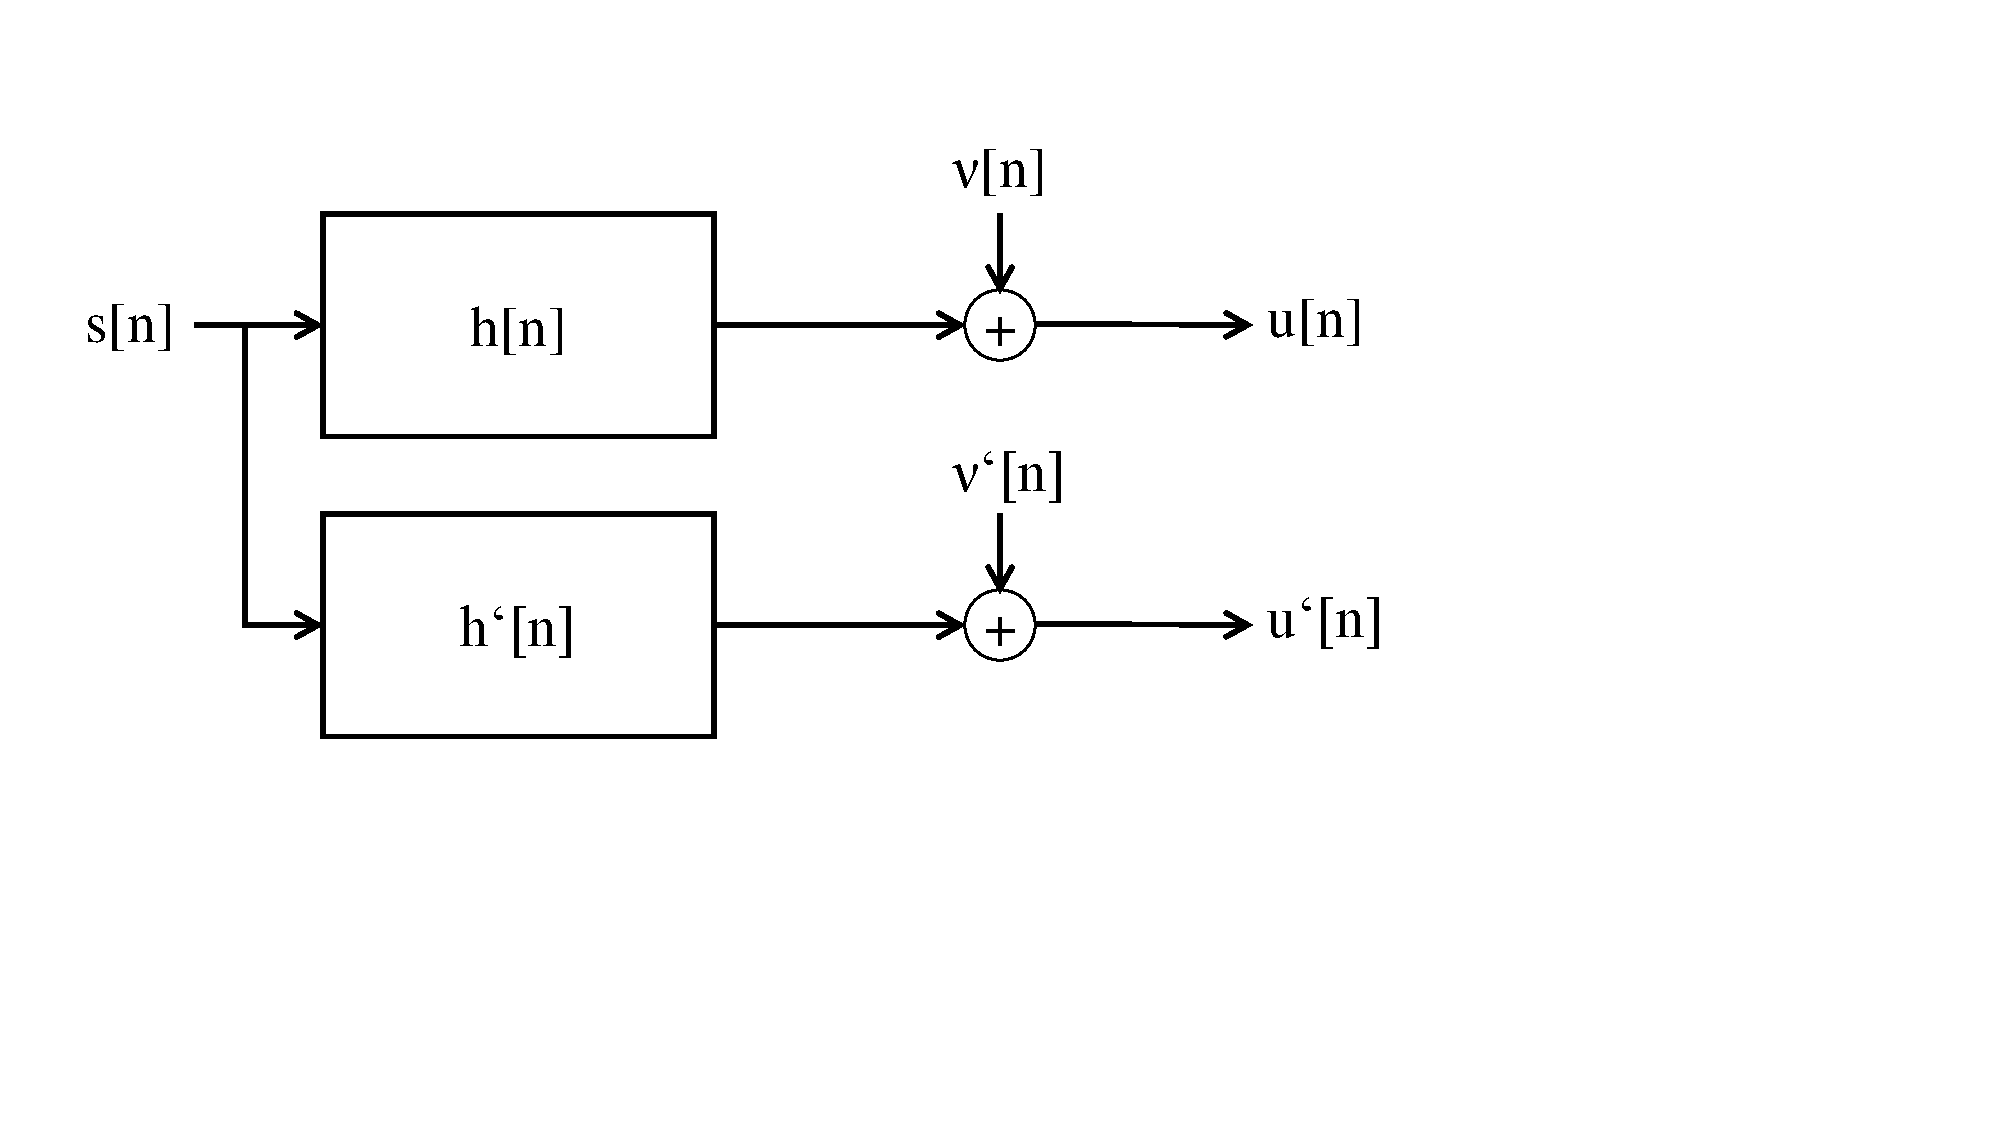
\includegraphics[trim =1cm 5cm 5cm 2cm, clip, width=0.70\textwidth]{graphics/Block_diagram_2_antenna_RX.pdf}
	\caption{Block diagram of a receiver with two inputs (antennas)}
	\label{fig:Block_diagram_2_antenna_RX}
\end{figure}

$\vec{u}[n] = \ma{H} \vec{s}[n] + \vec{\nu}[n]$\\
$\vec{u}'[n] = \ma{H}' \vec{s}[n] + \vec{\nu}'[n]$\\
$\underbrace{\mat{\vec{u}[n]\\ \vec{u}'[n]}}_{\vec{\tilde{u}}[n]} = \underbrace{\mat{\ma{H}\\ \ma{H}'}}_{\ma{\tilde{H}}} \vec{s}[n] + \underbrace{\mat{\vec{\nu}[n]\\ \vec{\nu}'[n]}}_{\ma{\tilde{\nu}}[n]}$\\
$\vec{\tilde{u}}[n] = \ma{\tilde{H}} \vec{s}[n] + \vec{\tilde{\nu}}[n]; \qquad \ma{\tilde{H}}\in \mathbb{C}^{2M\times N}$\\
$\ma{\tilde{H}}$ could have more rows than columns:\\
$(\ma{\tilde{H}}\ma{\tilde{R}}_s\ma{\tilde{H}}^H)\in\mathbb{C}^{2M\times 2M}$\\
$\Rightarrow$ If $2M > N$ we have a problem with the rank.
\\ \ \\

\mybox{
\textbf{Sherman-Morrison-Woodburry Identity}\\
Given $\ma{A}\in\mathbb{C}^{M\times M},\, \text{rank} \ma{A}=M$ and $\ma{C}\in\mathbb{C}^{N\times N},\, \text{rank} \ma{C}=N$ and $\ma{B}\in\mathbb{C}^{M\times N}$ and $\ma{D}\in\mathbb{C}^{N\times M}$, then:\\
$(\ma{A}+\ma{B}\ma{C}\ma{D})^{-1} = \ma{A}^{-1} - \ma{A}^{-1}\ma{B}(\ma{C}^{-1}+\ma{D}\ma{A}^{-1}\ma{B})^{-1}\ma{D}\ma{A}^{-1}$
}\\

\textbf{Proof:}\\
$(\ma{A}^{-1} - \ma{A}^{-1}\ma{B}(\ma{C}^{-1}+\ma{D}\ma{A}^{-1}\ma{B})^{-1}\ma{D}\ma{A}^{-1})(\ma{A}+\ma{B}\ma{C}\ma{D})$\\
$=\underbrace{\ma{A}^{-1}\ma{A}}_{\ma{I}} + \ma{A}^{-1}\ma{B}\ma{C}\ma{D} - \ma{A}^{-1}\ma{B}(\ma{C}^{-1}+\ma{D}\ma{A}^{-1}\ma{B})^{-1}\ma{C}^{-1}\ma{C}\ma{D}\underbrace{\ma{A}^{-1}\ma{A}}_{\ma{I}}-\ma{A}^{-1}\ma{B}(\ma{C}^{-1}+\ma{D}\ma{A}^{-1}\ma{B})^{-1}\ma{D}\ma{A}^{-1}\ma{B}\ma{C}\ma{D}$\\
$=\ma{I} + \ma{A}^{-1}\ma{B}(\ma{I}\underbrace{-(\ma{C}^{-1}+\ma{D}\ma{A}^{-1}\ma{B})^{-1}\ma{C}^{-1}-(\ma{C}^{-1}+\ma{D}\ma{A}^{-1}\ma{B})^{-1}\ma{D}\ma{A}^{-1}\ma{B}}_{-\underbrace{(\ma{C}^{-1}+\ma{D}\ma{A}^{-1}\ma{B})^{-1}(\ma{C}^{-1}+\ma{D}\ma{A}^{-1}\ma{B})}_{\ma{I}}})\ma{C}\ma{D}$\\
$=\ma{I}$\qed\\ \ \\

Applying the Sherman-Morrison-Woodburry Identity on $\vec{w}_{opt}$ with $\ma{B}=\ma{H}$, $\ma{C}=\ma{R}_s$, $\ma{D}=\ma{H}^H$ and $\ma{A}=\ma{R}_{\nu}$ we get:\\
\begin{flalign*}
\vec{w}_{opt}&=(\ma{H}\ma{R}_s\ma{H}^H+\ma{R}_{\nu})^{-1}\ma{H}\ma{R}_s\vec{e}_{l+1}&&\\
&=(\ma{R}_{\nu}^{-1} - \ma{R}_{\nu}^{-1}\ma{H}(\ma{R}_s^{-1}+\ma{H}^H\ma{R}_{\nu}^{-1}\ma{H})^{-1}\ma{H}^H\ma{R}_{\nu}^{-1})\ma{H}\ma{R}_s\vec{e}_{l+1}&&\\
&=\ma{R}_{\nu}^{-1}\ma{H}(\underbrace{\ma{I}}_{(\ma{R}_{s}^{-1}+\ma{H}^H\ma{R}_{\nu}^{-1}\ma{H})^{-1}(\ma{R}_{s}^{-1}+\ma{H}^H\ma{R}_{\nu}^{-1}\ma{H})}(-(\ma{R}_{s}^{-1}+\ma{H}^H\ma{R}_{\nu}^{-1}\ma{H})^{-1}\ma{H}^H\ma{R}_{\nu}^{-1}\ma{H})\ma{R}_{s}\vec{e}_{l+1}&&\\
&=\ma{R}_{\nu}^{-1}\ma{H}(\ma{R}_{s}^{-1}+\ma{H}^H\ma{R}_{\nu}^{-1}\ma{H})^{-1}\underbrace{(\ma{R}_s^{-1}+\underbrace{\ma{H}^H\ma{R}_{\nu}^{-1}\ma{H}-\ma{H}^H\ma{R}_{\nu}^{-1}\ma{H}}_{=0})\ma{R_s}}_{=\ma{I}}\vec{e}_{l+1}
\end{flalign*}
\mybox{
\begin{flalign}
\vec{w}_{opt}&=\ma{R}_{\nu}^{-1}\ma{H}\underbrace{(\ma{R}_s^{-1}+\ma{H}^H\ma{R}_{\nu}^{-1}\ma{H})^{-1}}_{N\times N}\vec{e}_{l+1}&&\label{eq:wopt_1}\\
&=\underbrace{(\ma{R}_{\nu}+\ma{H}\ma{R}_{s}\ma{H}^H)^{-1}}_{M\times M}\ma{H}\ma{R}_s\vec{e}_{l+1}\label{eq:wopt_2}
\end{flalign}
}
$\ma{H}\in\mathbb{C}^{M\times N}$\\
If $M<N$ use equation \eqref{eq:wopt_2}: $M$ equations in $M$ unknowns\\
If $N<M$ use equation \eqref{eq:wopt_1}: $N$ equations in $N$ unknowns\\
\textbf{Note: processor \& memory load}\\
$\ma{A}\vec{x}=\vec{b}:\quad \ma{A}\in\mathbb{C}^{n\times n}$\\
\begin{tabular}{ll}
Solve for \vec{x}: &computational load $\sim n^3$\\
&memory $\sim n^2$\\
\end{tabular}
\end{doublespace}

\begin{doublespace}
\textbf{Note: Inter-Symbol-Interference}\\
$y[n]=\vec{w}^H\vec{u}[n] = \vec{w}(\ma{H}\vec{s}[n]+\vec{\nu}[n]) = \vec{w}^H(\underbrace{\mat{\vec{h}_1&\vec{h}_2&\shdots&\vec{h}_N}}_{\ma{H}}\underbrace{\vec{s}[n]}_{\mat{s[n]\\s[n-1]\\\svdots\\s[n-M+1]}}+\vec{\nu}[n])$\\
$d[n]=s[n-l]$\\
$y[n]=\vec{w}^H(\vec{h}_{l+1}\underbrace{\vec{s}[n-l]}_{\text{signal of interest}}+\underbrace{\sum\limits_{k=1; k\neq l+1}^{N}\vec{h}_k \vec{s}[n-k]}_{\text{Inter-Symbol-Interference}}+\underbrace{\vec{\nu}[n])}_{\text{Noise}}$\\
\subsection{Filter with different kinds of Noise}

\subsubsection{Special case: White Noise \& White Signal} 
$\ma{R}_s=\sigma_d^2\ma{I};\qquad \ma{R}_\nu=\sigma_\nu^2\ma{I}$\\
$\vec{w}_{opt}=(\frac{\sigma_u^2}{\sigma_d^2}\ma{I}+\ma{H}\ma{H}^H)^{-1}\ma{H}\vec{e}_{l+1}$\\
\\
\subsubsection{Case 1: High SNR (signal to noise ratio)}
$\ma{H}\in\mathbb{C}^{M\times N}; \qquad M<N$\\
$\text{rank}\ma{H}=M$ (full rank \ma{H})\\
$\ma{H}=\ma{U}_1\ma{\Sigma}_1\ma{V}_1^H \underbrace{=}_{\text{rank}\ma{H}=M} \ma{U}\ma{\Sigma}_1\ma{V}_1^H$
\begin{flalign*}
(\ma{H}\ma{H}^H)^{-1}\ma{H} &= (\ma{U}\ma{\Sigma}_1\ma{V}_1^H\ma{V}_1\ma{\Sigma}_1\ma{U}^H)^{-1}\ma{U}\ma{\Sigma}_1\ma{V}_1^H&&\\
&=(\ma{U}\ma{\Sigma}_1^2\ma{U}^H)^{-1}\ma{U}\ma{\Sigma}_1\ma{V}_1^H&&\\
&=\ma{U}\ma{\Sigma}_1^{-2}\underbrace{\ma{U}^H\ma{U}}_{\ma{I}}\ma{\Sigma}_1\ma{V}_1^H&&\\
&=\ma{U}\ma{\Sigma}_1^{-1}\ma{V}_1^H=\ma{U}_1\ma{\Sigma}_1^{-1}\ma{V}_1^H=(\ma{V}_1\ma{\Sigma}_1^{-1}\ma{U}^H)^H&&\\
&=(\ma{H}^+)^H = (\ma{H}^H)^+
\end{flalign*}
$\lim\limits_{\frac{\sigma_d^2}{\sigma_\nu^2}\rightarrow\infty}\vec{w}_{opt}=(\ma{H}\ma{H}^H)^{-1}\ma{H}\vec{e}_{l+1}=\underbrace{(\ma{H}^H)^+}_{\text{Moore-Penrose-Pseudo-Inverse}}\vec{e}_{l+1}$\\ \\
No optimal solution because:\\
Try: $\vec{w}^H\ma{H}\stackrel{!}{=}\vec{e}_{l+1}^T;\quad y[n]=\underbrace{\vec{w}^H\ma{H}}_{\vec{e}_{l+1}^T}\vec{s}[n]=\vec{s}[n-1]$\\
However it does not work!\\
$\ma{H}^H\vec{w}=\vec{e}_{l+1}$\\
$\ma{H}^H\in\mathbb{C}^{N\times M}\qquad \text{with } M<N$\\
Number of degrees of freedom = $M$\\
Number of constraints = $N>M$\\
$\Rightarrow$ No exact solution exists!\\
$\Rightarrow$ LS-Solution (least square)\\
\mybox{
$\vec{w}_{LS}=(\ma{H}^H)^+\vec{e}_{l+1}$}
\mybox{
For high SNR the optimum filter tries to suppress the interference but lack DoF (Degrees of Freedom) to do it perfectly.\\
$\vec{w}_{LS}=\arg\min\limits_{\vec{w}}||\vec{w}^H\ma{H}-\vec{e}_{l+1}||_2^2$\\
}\\
The higher the dimensions, the better the outcome of the filter. \\ \ \\
\textbf{Work-around: Block processing}\\
at Tx: pre-pend K guard symbols\\
at Rx: discard first K received symbols\\
\textbf{Example:}\\
$K=2$ (number of \textcolor[rgb]{1,0,0}{guard symbols}), $\quad M=4$ (number of payload symbols)\\
$\mat{u[n]\\u[n-1]\\u[n-2]\\u[n-3]}=\vec{\nu}[n] + \mat{h_0&h_1&h_2&0&0&0\\ 0&h_0&h_1&h_2&0&0\\ 0&0&h_0&h_1&h_2&0\\ 0&0&0&h_0&h_1&h_2}\mat{s[n]\\s[n-1]\\s[n-2]\\s[n-3]\\\textcolor[rgb]{1,0,0}{s[n]}\\\textcolor[rgb]{1,0,0}{s[n-1]}}$\\
$\ma{\overset{\circ}{H}}=\mat{h_0&h_1&h_2&0\\ 0&h_0&h_1&h_2\\ h_2&0&h_0&h_1\\ h_1&h_2&0&h_0}$ (cyclic matrix)\\
$\ma{\overset{\circ}{H}}$ is invertible \pfeil with no noise, we get a perfect solution with losing bandwidth efficiency\\
$\vec{s}[n] = \mat{s[n]\\s[n-1]\\s[n-2]\\s[n-3]}$\\
Example MATLAB-code: \lstinline !Q=fft(eye(M))/sqrt(M)!\\
$\ma{Q}^H\mat{H}\mat{Q}=\mat{a_1& & & \\ &a_2& & \\ & &a_3& \\ & & &a_4}$\\
$\mat{a_1&a_2&a_3&a_4}=\text{fft}(\mat{h_0&h_1&h_2&0}) \Rightarrow$ OFDM (Orthogonal Frequency Division Multiplexing)\\ \ \\

\subsubsection{Case 2: Low SNR (High Noise)}
$\frac{\sigma_\nu^2}{\sigma_d^2}\rightarrow\infty$\\
$y[n]\approx\vec{w}^H(\vec{h}_{l+1}s[n-l]+\vec{\nu}[n])$\\
$SNR=\frac{E[|y[n]|^2|\vec{\nu}[n]=\vec{0}]}{E[|y[n]|^2|s[n-l]=0]} = \frac{\sigma_d^2|\vec{w}^H\vec{h}_{l+1}|^2}{\sigma_\nu^2\vec{w}^H\vec{w}}$\\

\textbf{Calculation of the SNR with respect to variances of signal and noise}\\
System: $y[n]=\vec{w}^H\vec{u}[n]=\vec{w}^H\ma{H}\vec{s}[n]+\vec{w}^H\vec{\nu}[n]$\\
\with $\vec{s}[n]=\vec{e}_{l+1}\cdot d[n]$

\parbox{0.5\textwidth}{
\begin{align*}
&E[|y[n]|^2|\vec{\nu}[n]=\vec{0}]\\
=& E[(\vec{w}^H\ma{H}\vec{s}[n])^*(\vec{w}^H\ma{H}\vec{s}[n])]\\
=& E[(\vec{s}[n]^H\ma{H}^H\vec{w})(\vec{w}^H\ma{H}\vec{s}[n])]\\
=& E[\vec{s}[n]^H\ma{H}^H\vec{w}\vec{w}^H\ma{H}\vec{s}[n]]\\
=&E[d[n]^*d[n]\cdot\vec{e}_{l+1}^H\ma{H}^H\vec{w}\vec{w}^H\ma{H}\vec{e}_{l+1}]\\
=&E[\abs{d[n]}^2\cdot\underbrace{\vec{h}_{l+1}^H\vec{w}}_{\in\mathbb{C}^{1\times 1}}\underbrace{\vec{w}^H\vec{h}_{l+1}}_{\in\mathbb{C}^{1\times 1}}]\\
=& E[\underbrace{\abs{d[n]}^2}_{\text{random}}\cdot\underbrace{\abs{\vec{w}^H\vec{h}_{l+1}}^2}_{\text{deterministic}}]\\
=& E[\abs{d[n]}^2]\cdot\abs{\vec{w}^H\vec{h}_{l+1}}^2]\\
=& \sigma_d^2\cdot\abs{\vec{w}^H\vec{h}_{l+1}}^2\\
\end{align*}
}
\parbox{0.5\textwidth}{
\begin{align*}
&E[|y[n]|^2|s[n-l]=0]\\
=&E[(\vec{w}^H\vec{\nu}[n])^*(\vec{w}^H\vec{\nu}[n])]\\
=&E[(\vec{w}^H\vec{\nu}[n])^H(\vec{w}^H\vec{\nu}[n])]\\
=&E[\vec{\nu}[n]^H\vec{w}\vec{w}^H\vec{\nu}[n]]\\
=&E[\tr(\vec{\nu}[n]^H\vec{w}\vec{w}^H\vec{\nu}[n])]\\
=&E[\tr(\vec{w}^H\vec{\nu}[n]\vec{\nu}[n]^H\vec{w})]\\
=&\tr(\vec{w}^H E[\vec{\nu}[n]\vec{\nu}[n]^H]\vec{w})\\
=&\tr(\vec{w}^H(\sigma_\nu^2 \ma{I})\vec{w})\\
=&\sigma_\nu^2\cdot\tr(\underbrace{\vec{w}^H\vec{w}}_{\in\mathbb{C}^{1\times 1}})=\sigma_\nu^2\cdot\vec{w}^H\vec{w}\\
\end{align*}}

\textbf{Mathematical derivation of Cauchy-Schwarz-Inequality:}\\
$\vec{z}:=\vec{h}-\vec{w}\frac{\vec{w}^H\vec{h}}{\vec{w}^H\vec{w}}$
\begin{flalign*}
\vec{z}^H\vec{z}&=(\vec{h}^H-\frac{\vec{h}^H\vec{w}}{\vec{w}^H\vec{w}}\vec{w})(\vec{h}-\vec{w}\frac{\vec{w}^H\vec{h}}{\vec{w}^H\vec{w}})&&\\
&=\vec{h}^H\vec{h}-\frac{(\vec{h}^H\vec{w})(\vec{w}^H\vec{h})}{\vec{w}^H\vec{w}}-\frac{(\vec{h}^H\vec{w})(\vec{w}^H\vec{h})}{\vec{w}^H\vec{w}}+\frac{(\vec{h}^H\vec{w})(\vec{w}^H\vec{h})\vec{w}^H\vec{w}}{(\vec{w}^H\vec{w})(\vec{w}^H\vec{w})}&&\\
&=\vec{h}^H\vec{h}-\frac{|\vec{w}^H\vec{h}|^2}{\vec{w}^H\vec{w}}\geq 0
\end{flalign*}
\mybox{
Cauchy-Schwarz-Inequality:\\
$\frac{|\vec{w}^H\vec{h}|^2}{\vec{w}^H\vec{w}}\leq\vec{h}^H\vec{h}$
}
$SNR=\frac{\sigma_d^2}{\sigma_\nu^2}\frac{|\vec{w}^H\vec{h}_{l+1}|^2}{\vec{w}^H\vec{w}}\leq\frac{\sigma_d^2}{\sigma_\nu^2}\vec{h}_{l+1}^H\vec{h}_{l+1}$\\
$\vec{w}_{MF}=\arg\max\limits_{\vec{w}}SNR=\const \cdot \vec{h}_{l+1}\with \const\neq 0\qquad$ where MF stands for "matched filter"\\
try: $SNR\left.\right|_{\vec{w}=\vec{w}_{MF}}=\frac{\sigma_d^2}{\sigma_\nu^2}\frac{\left|\vec{h}_{l+1}^H\vec{h}_{l+1}\right|^2\cdot|\const|^2}{\vec{h}_{l+1}^H\vec{h}_{l+1}\cdot|\const|^2}=\frac{\sigma_d^2}{\sigma_\nu^2}\vec{h}_{l+1}^H\vec{h}_{l+1}$\\
$\vec{w}=\vec{w}_{MF}$ achieves an upper bound of the SNR.\\
\mybox{
Optimum Filter Solution:\\
$\vec{w}_{opt}=\underbrace{\frac{\sigma_d^2}{\sigma_\nu^2}}_{\const}\vec{h}_{l+1}=\vec{w}_{MF}$}
$\lim\limits_{\frac{\sigma_d^2}{\sigma_\nu^2}\rightarrow0}\vec{w}_{opt}=\vec{w}_{MF}\sim\vec{h}_{l+1}$
\end{doublespace}

\subsection{Steepest Descent Algorithm (SDA)}
$\vec{w}_{opt}=\ma{R}^{-1}\vec{p},\qquad \ma{R}\vec{w}_{opt}=\vec{p}$\\
One method to solve this problem woulbd be the Gauß-Elimination but since \ma{R} and \vec{p} usually change it is neccessary to recalulate everything when ever something changes. This would lead to an enormouse effort. So an iterative solution would be more productive.\\
\textbf{Iterative solution:}\\
\begin{doublespace}
$\vec{w}[n+1]=\vec{w}[n]+\Delta\vec{w}[n]$\\
$J=\sigma_d^2-\vec{w}^H\vec{p}-\vec{p}^H\vec{w}+\vec{w}^H\ma{R}\vec{w};\quad \ma{R}>\vec{0}; \qquad \ma{R}=\ma{R}^H$\\
$dJ=\left(\frac{\partial J}{\partial \vec{w}}\right)^T d\vec{w} + \left(\frac{\partial J}{\partial \vec{w^*}}\right)^T d\vec{w}^*$\\
\with $\left(\frac{\partial J}{\partial \vec{w}}\right)^T d\vec{w} = \left(\left(\frac{\partial J^*}{\partial \vec{w^*}}\right)^T d\vec{w}^*\right)^*\underbrace{=}_{J\underbrace{=}_{J\in\mathbb{R}}J^*}\left(\left(\frac{\partial J}{\partial \vec{w^*}}\right)^T d\vec{w}^*\right)^*$ we get:\\
$dJ=2\Re{\left(\frac{\partial J}{\partial \vec{w}^*}\right)^T d\vec{w}^*}$\\
$dJ=2\Re{\left(\frac{\partial J}{\partial \vec{w}^*}\right)^H d\vec{w}} \leq 2 \left|\left(\frac{\partial J}{\partial \vec{w}^*}\right)^H d\vec{w}\right|$\\
$d\vec{w}=\frac{\partial J}{\partial\vec{w}^*}\cdot \const^*;\qquad \const<0$\\
$\Delta\vec{w}[n]=-\mu\frac{\partial J}{\partial\vec{w}^*[n]};\qquad \mu>0$\\
$\frac{\partial J}{\partial \vec{w}^*[n]}=-\vec{p}+\ma{R}\vec{w}[n]$\\
\begin{flalign*}
\vec{w}[n+1]&=\vec{w}[n]+\Delta\vec{w}[n] = \vec{w}[n]-\mu\left(\vec{p}+\ma{R}\vec{w}[n]\right);\qquad \mu>0&&\\
&=(\ma{I}-\mu\ma{R})\vec{w}[n]+\mu\vec{p}
\end{flalign*}

Does $\vec{w}[n],\,\vec{w}[n+1],\ldots$ converge to $\vec{w}_{opt}$?\\
$\vec{c}[n]=\vec{w}[n]-\vec{w}_{opt}$\\
$\underbrace{c[n+1]+\vec{w}_{opt}}_{=\vec{w}[n+1]}=(\ma{I}-\mu\ma{R})\underbrace{\vec{c}[n]+\vec{w}_{opt}}_{\vec{w}[n]}+\mu\vec{p}$\\
$c[n+1]=(\ma{I}-\mu\ma{R})\vec{c}[n]-\underbrace{\mu\ma{R}\overbrace{\vec{w}_{opt}}^{\ma{R}^{-1}\vec{p}}+\mu\vec{p}}_{=\vec{0}}$\\
\mybox{
$c[n+1]=(\ma{I}-\mu\ma{R})\vec{c}[n]$
}\\
Does $c[n],\,c[n+1],\,\ldots$ converge to \vec{0}?\\
EVD: $\ma{R}=\ma{Q}\ma{\Lambda}\ma{Q}^{-1}\underbrace{=}_{\ma{R}=\ma{R}^H}\ma{Q}\ma{\Lambda}\ma{Q}^{H}$\\
$\ma{\Lambda}=\mat{\lambda_1&&&&\\&\lambda_2&&&\\&&\lambda_3&&\\&&&\ddots&\\&&&&\lambda_M};\quad \lambda_i>0;\quad i\in \{1,2,\ldots,M\};\qquad (\ma{R}>0)$\\
\begin{flalign*}
\vec{c}[n+1]&=(\ma{I}-\mu\underbrace{\ma{Q}\ma{\Lambda}\ma{Q}^{H}}_{=\ma{R}})\vec{c}[n]=(\underbrace{\ma{Q}\ma{Q}^H}_{=\ma{I}}-\mu\ma{Q}\ma{\Lambda}\ma{Q}^{H})\vec{c}[n]&&\\
&=\ma{Q}(\ma{I}-\mu\ma{\Lambda})\ma{Q}^H\vec{c}[n]
\end{flalign*}
$\underbrace{\ma{Q}^H\vec{c}[n+1]}_{\vec{z}[n+1]}=(\ma{I}-\mu\ma{\Lambda})\underbrace{\ma{Q}^H\vec{c}[n]}_{\vec{z}[n]}$\\
\mybox{
$\vec{z}[n+1]=(\ma{I}-\mu\ma{\Lambda})\vec{z}[n]$
}\\
$\vec{z}[n]=\mat{z_1[n]&z_2[n]&\shdots&z_M[n]}^T$\\
\mybox{
$z_k[n+1]=(1-\mu\lambda_k)z_k[n];\qquad 1\leq k\leq M$
}\\
$z_k[n],\,z_k[n+1]\ldots$ converge to 0 if and only if $\left|1-\mu\lambda_k\right|<1;\qquad \forall k$\\
\textbf{case 1:} $1-\mu\lambda_k\geq 0\qquad \left[\mu\leq \frac{1}{\lambda_k}\right]$
\begin{flalign*}
\text{then }1-\mu\lambda_k&<1&&\\
-\mu\lambda_k&<0; \qquad \mu>0,\quad \lambda_l>0&&\\
-\mu&<0&&\\
\mu&>0
\end{flalign*}
\mybox{
$0<\mu\leq\frac{1}{\lambda_k}$
}\\ \ \\
\textbf{case 2:} $1-\mu\lambda_k\leq 0\qquad \left[\mu\geq \frac{1}{\lambda_k}\right]$
\begin{flalign*}
\text{then }-1+\mu\lambda_k&<1&&\\
\mu\lambda_k&<2&&\\
\mu&<\frac{2}{\lambda_k}
\end{flalign*}
\mybox{
$\frac{1}{\lambda_k}\leq\mu\leq\frac{2}{\lambda_k}$
}
\mybox{
\textbf{Case 1 \& Case 2:}\\
$\Rightarrow 0<\mu<\frac{2}{\lambda_k} \Leftrightarrow z_k[n],\,z_k[n+1],\,\ldots$ converges to 0.}\\ \ \\
\mybox{
\textbf{Key results:}\\
$\vec{w}[n],\,\vec{w}[n+1],\ldots$ converge to $\vec{w}_{opt}$ iff\\
$0\leq\mu\leq\frac{2}{\lambda_{max}} \qquad \lambda_{max}=\text{ maximum Eigenvalue of }\ma{R}$
}\\ \\
\textbf{Computation of $\lambda_{max}$ is costly!}\\
$\underbrace{\sum\limits_{k=1}^M\lambda_k}_{\text{tr}\ma{R}} > \lambda_{max} < \tr\ma{R}$\\
$0<\mu<\frac{2}{\text{tr}\ma{R}}<\frac{2}{\lambda_{max}}$\\
\end{doublespace}
$\text{tr}\ma{R}$ is cheap to compute. Therfor in practice  $0<\mu<\frac{2}{\text{tr}\ma{R}}$ can be used. This is sufficeint for convergence. But usually one is interested in using an optimum step-size $\mu$ to achive optimum performance of the algorithm.

\subsubsection{Optimum step-size \texorpdfstring{$\mu$}{}}
\begin{figure}[H]
	\centering
		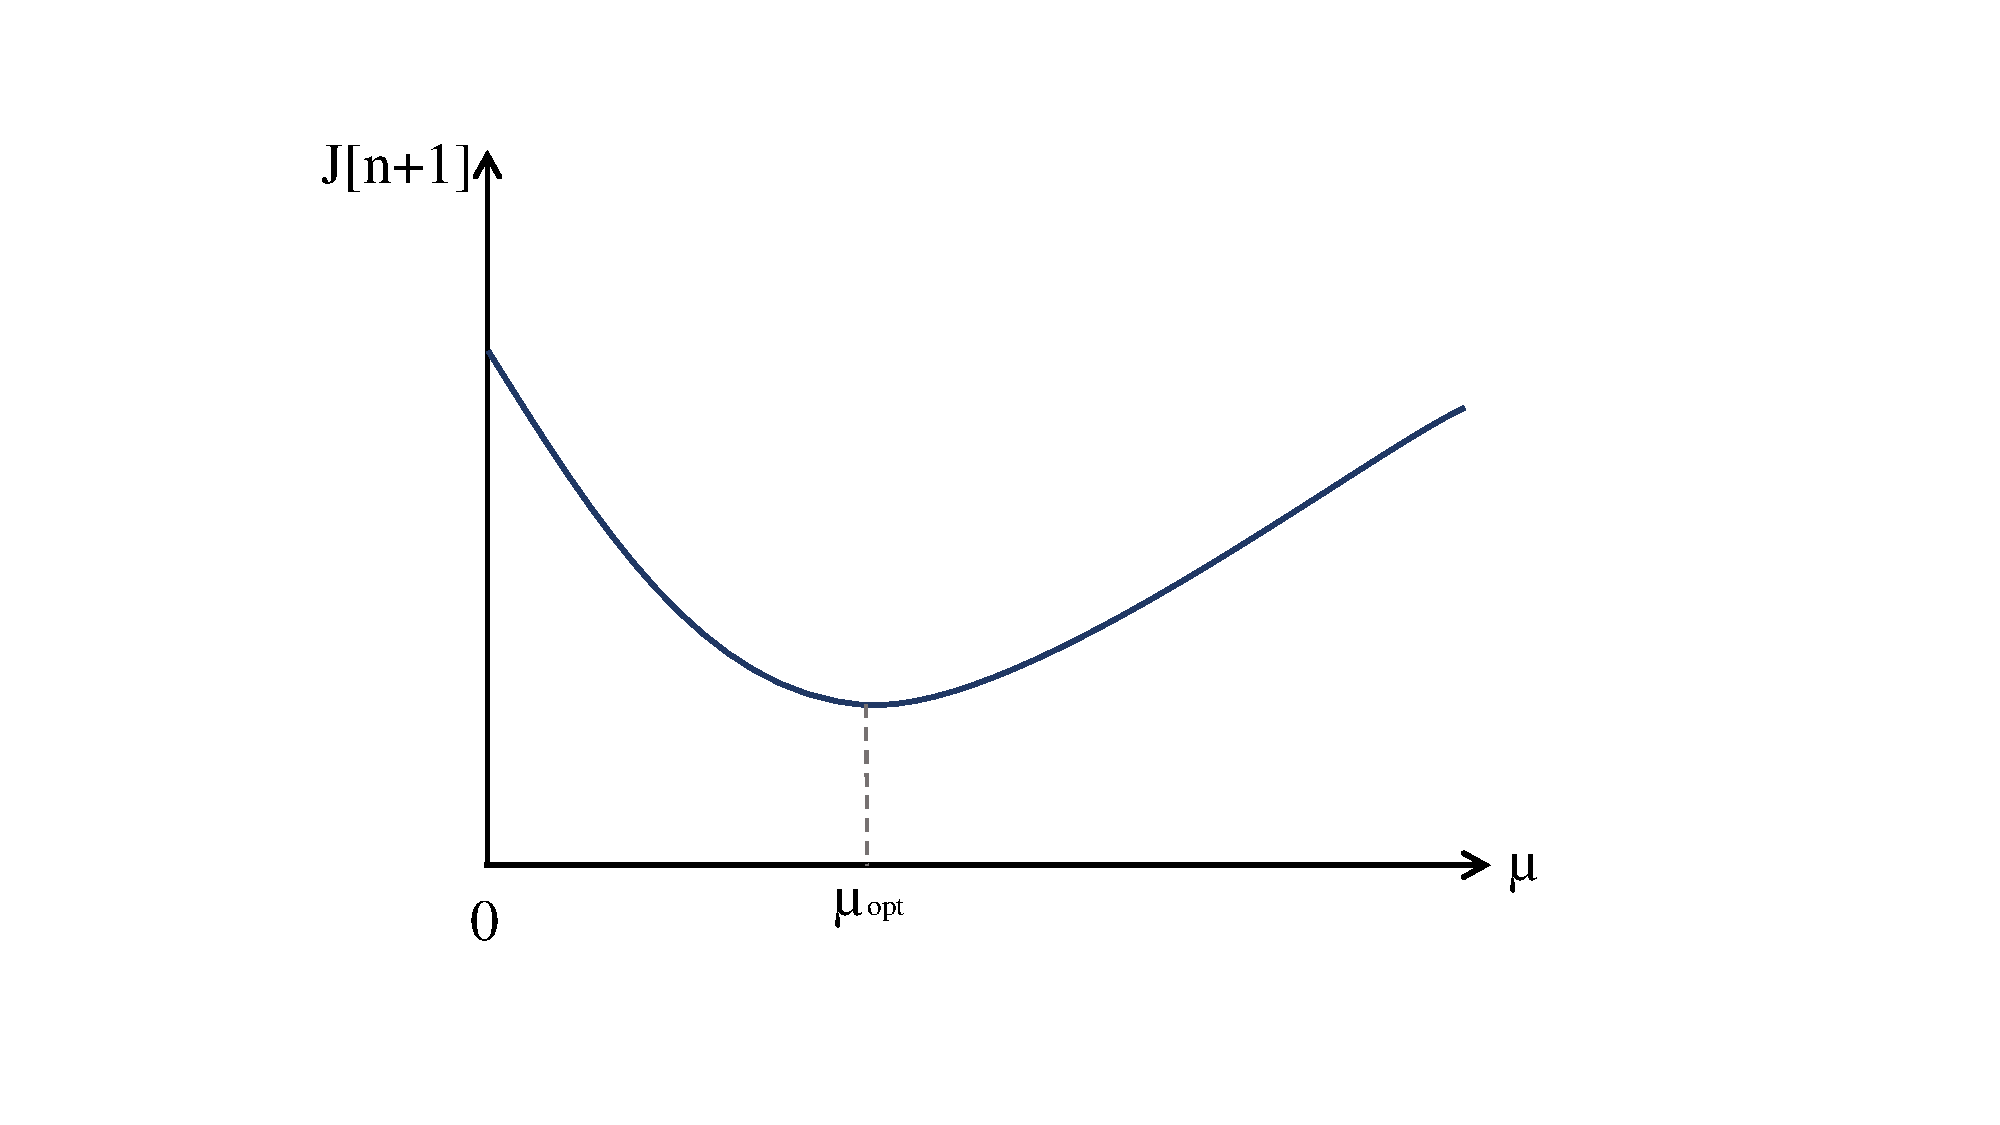
\includegraphics[trim =1cm 3cm 5cm 2cm, clip, width=0.70\textwidth]{graphics/Optimum_step_size_examplepdf.pdf}
	\caption{Example characteristics of the cost function $J[n+1]$ plotted over the step-size $\mu$}
	\label{fig:Optimum_step_size_examplepdf}
\end{figure}
\begin{doublespace}
Solve $\frac{\partial J[n+1]}{\partial \mu^*}=0$ for $\mu=\mu_{opt}$:\\
$J[n+1]=\sigma_d^2-\vec{P}^H\vec{w}[n+1]-\vec{w}^H[n+1]\vec{P}+\vec{w}^H[n+1]\ma{R}\vec{w}[n+1]$\\
$\vec{w}[n+1]=\vec{w}[n]+\mu\vec{r}[n]\quad$ with $\vec{r}[n]=\vec{p}-\ma{R}\vec{w}[n]$\\
\mybox{
$\mu_{opt}=\frac{\vec{r}^H[n]\vec{r}[n]}{\vec{r}^H[n]\ma{R}\vec{r}[n]}$
}
Note: The optimum step-size $\mu_{opt}$ is (usually) different for each step.
\end{doublespace}

\subsubsection{Summary: Steepest Descent Algorithm}\mybox{
Find the optimal $\vec{w}_{opt}$ for $\ma{R}\vec{w}=\vec{p}$\\
\textbf{Input:} $\ma{R}=\ma{R}^H>\vec{0}, \qquad \vec{p}$\\
\begin{tabular}{ll}
\textbf{Output:} &\vec{w} that solves $\ma{R}\vec{w}=\vec{p}$ approximately.\\
&This \vec{w} is the minimum of $J=\sigma_d^2-\vec{w}^H\ma{R}-\vec{p}^H\vec{w}+\vec{w}^H\ma{R}\vec{w}$\\
\end{tabular}\\
\textbf{Algorithm:}\\
\begin{tabular}{ll}
	1. Init: &$\vec{w}\leftarrow 0$\\
	2. Iteration: &$\vec{r}\leftarrow \vec{p}-\ma{R}\vec{w}$\\
	&$\mu\leftarrow\frac{\vec{r}^H\vec{r}}{\vec{r}^H\ma{R}\vec{r}}$\\
	&$\vec{w}\leftarrow\vec{w}+\mu\vec{r}$\\
  3. Go to step 2 until $\vec{r}^H\vec{r}<\varepsilon$\\
\end{tabular}}
\\ \ \\
\begin{table}[H]
\begin{center}
\begin{tabular}{l|l}
with optimum $\mu$& fixed $\mu$\\
\hline
$4M^2+5M$&$2M^2+4M$\\
\end{tabular}
\end{center}
\caption{Number of operations ($\cdot,\,+$) per iteration}
\label{tab:SDA_no_operaion_per_iteration}
\end{table}

\rule{\textwidth}{.4pt}\\
\textbf{MATLAB experiment to show the number of steps for optimum $\mu$:}\\
Random $\ma{R}\in\mathbb{C}^{M\times M}, \quad \ma{R}>0, \quad \frac{\lambda_{max}}{\lambda_{min}}\leq 10$\\
Random $\vec{p}\in\mathbb{C}^{M\times 1}$\\
Run SDA with optimum $\mu$, count interations\\
Repeat many times $\rightarrow$ \underline{median} iteartion number\\
\begin{table}[H]
\begin{center}
\begin{tabular}{c||c|c|c}
M&10&100&1000\\
\hline
number of iterations (median)&32&36&40\\
\end{tabular}
\end{center}
\caption{Results of MATLAB experiment to show the number of steps for optimum $\mu$}
\label{tab:res_numb_iter_vs_M}
\end{table}
$\Rightarrow$ number of iterations $=28+4\log_{10}M$\\
This algorithm is perfect for parallel computation\\
\rule{\textwidth}{.4pt}\\ \ \\

\textbf{Example: Linear Constrained Optimization}\\
$\min\vec{w}^H\ma{A}\vec{w}, \quad \text{s. t. } \ma{B}\vec{w}=\vec{c};\qquad \ma{A}>\vec{0}$\\
$\ma{B}=\mat{\ma{U}_1&\ma{U}_2}\cdot \mat{\ma{\Sigma}_1&\ma{0}\\\ma{0}&\ma{0}}\cdot \mat{\ma{V}_1^H\\\ma{V}_2^H}$\\
with $\ma{B}\in\mathbb{C}^{q\times M},\quad \ma{\Sigma}_1\in\mathbb{C}^{q\times q}, \quad \ma{V}_1^H\in\mathbb{C}^{q\times M} \text{ and } \ma{V}_2^H\in\mathbb{C}^{(M-q)\times M}$\\
$q\leq M;\qquad \nullsp\ma{B}=\text{im}\ma{V}_2$\\
$\rank\ma{B}=q$\\
 
$\ma{B}\vec{w}=\vec{c}:\quad \vec{w}\in\left\{\underbrace{\ma{B}^+\vec{c}}_{\vec{w}_q}-\ma{V}_2\vec{w}_a\left.\right|\vec{w}_a\in\mathbb{C}^{(M-q)\times 1}\right\}$\\
$\vec{w}=\vec{w}_q-\ma{V}_2\vec{w}_a$\\
$\vec{w}_q$ is the optimum solution. It is a particular solution of the linear equation system. Under constraint equation system\\
$\vec{w}_a$ is used to project the null space \\

\begin{flalign*}
\vec{w}^H\ma{A}\vec{w}&=(\vec{w}_q^H-\vec{w}_a^H\ma{V}_2^H)\ma{A}(\vec{w}_q-\ma{V}_2\vec{w}_a)&&\\
&=\underbrace{\vec{w}_q^H\ma{A}\vec{w}_q}_{\sigma_d^2} - \underbrace{\vec{w}_q^H\ma{A}\ma{V}_2}_{\vec{p}^H}\vec{w}_a - \vec{w}_a^H\underbrace{\ma{V}_2^H\ma{A}\vec{w}_q}_{\vec{p}} + \vec{w}_a^H\underbrace{\ma{V}_2^H\ma{A}\ma{V}_2}_{\ma{R}}\vec{w}_a&&\\
&=\sigma_d^2-\vec{p}^H\vec{w}_a - \vec{w}_a^H\vec{p} + \vec{w}_a^H\ma{R}\vec{w}_a
\end{flalign*}
\pfeil substitution for iterative algorithm

Optimization of the cost function with respect to $\vec{w}_a \, (\ma{V}_2)$, which represents the nullspace of the constraints.

\begin{flalign*}\\
\frac{\partial }{\partial \vec{w}_a^*}\left(\vec{w}^H\ma{A}\vec{w}\right)=&\frac{\partial }{\partial \vec{w}_a^*}\left(
\vec{w}_q^H\ma{A}\vec{w}_q-\vec{w}_q^H\ma{A}\ma{V}_2\vec{w}_a-\vec{w}_a^H\ma{V}_2^H\ma{A}\vec{w}_q+\vec{w}_a^H\ma{V}_2^H\ma{A}\ma{V}_2\vec{w}_a\right)\\
=&-\underbrace{\ma{V}_2^H\ma{A}\vec{w}_q}_{\vec{p}}+\underbrace{\ma{V}_2^H\ma{A}\ma{V}_2}_{\ma{R}}\vec{w}_a
\overset{!}{=}0
\end{flalign*}

Is the same Problem as we already solved with the SDA ($\ma{R}\vec{w}_a=\vec{p}$).

\begin{enumerate}
	\item Compute SVD of \ma{R}: $\vec{w}_q=\ma{B}^+\vec{c}; \quad \ma{V}_2;\qquad \ma{B}^+=\ma{V}_1\ma{\Sigma_1^{-1}}\ma{U}_1^H$
	\item $\ma{R} \leftarrow \ma{V}_2\ma{A}\ma{V}_2; \quad \vec{p}\leftarrow \ma{V}_2^H\ma{A}\vec{w}_q$
	\item Run SDA for $\vec{w}_a$
	\item $\vec{w} \leftarrow \vec{w}_q - \ma{V}_2\vec{w}_a$
\end{enumerate}

\subsubsection{Steepest Descent Procedure}
Procedure runs permanently with a exponential weighted estimation of correlation matrix and vector.\\
\begin{doublespace}
$\ma{R}=E[\vec{u}[n]\vec{u}^H[n]], \qquad \vec{p}=E[\vec{u}[n]d^*[n]]$\\
Problem: \ma{R} and \vec{p} are unknown and changing. Estimation and tracking is necessary.\\
$\rightarrow$ Averaging in \underline{time}.\\
Idea: $\ma{\hat{R}}[n]=\frac{1}{S}\sum\limits_{k=0}^{S-1}\vec{u}[n-k]\vec{u}^H[n-k]$\\
Generalize: $\ma{\hat{R}}[n]=\frac{\sum\limits_{k=0}^{\infty}a_k\vec{u}[n-k]\vec{u}^H[n-k]}{\sum\limits_{k=0}^{\infty}a_k}$\\
\end{doublespace}
\begin{figure}[H]
	\centering
		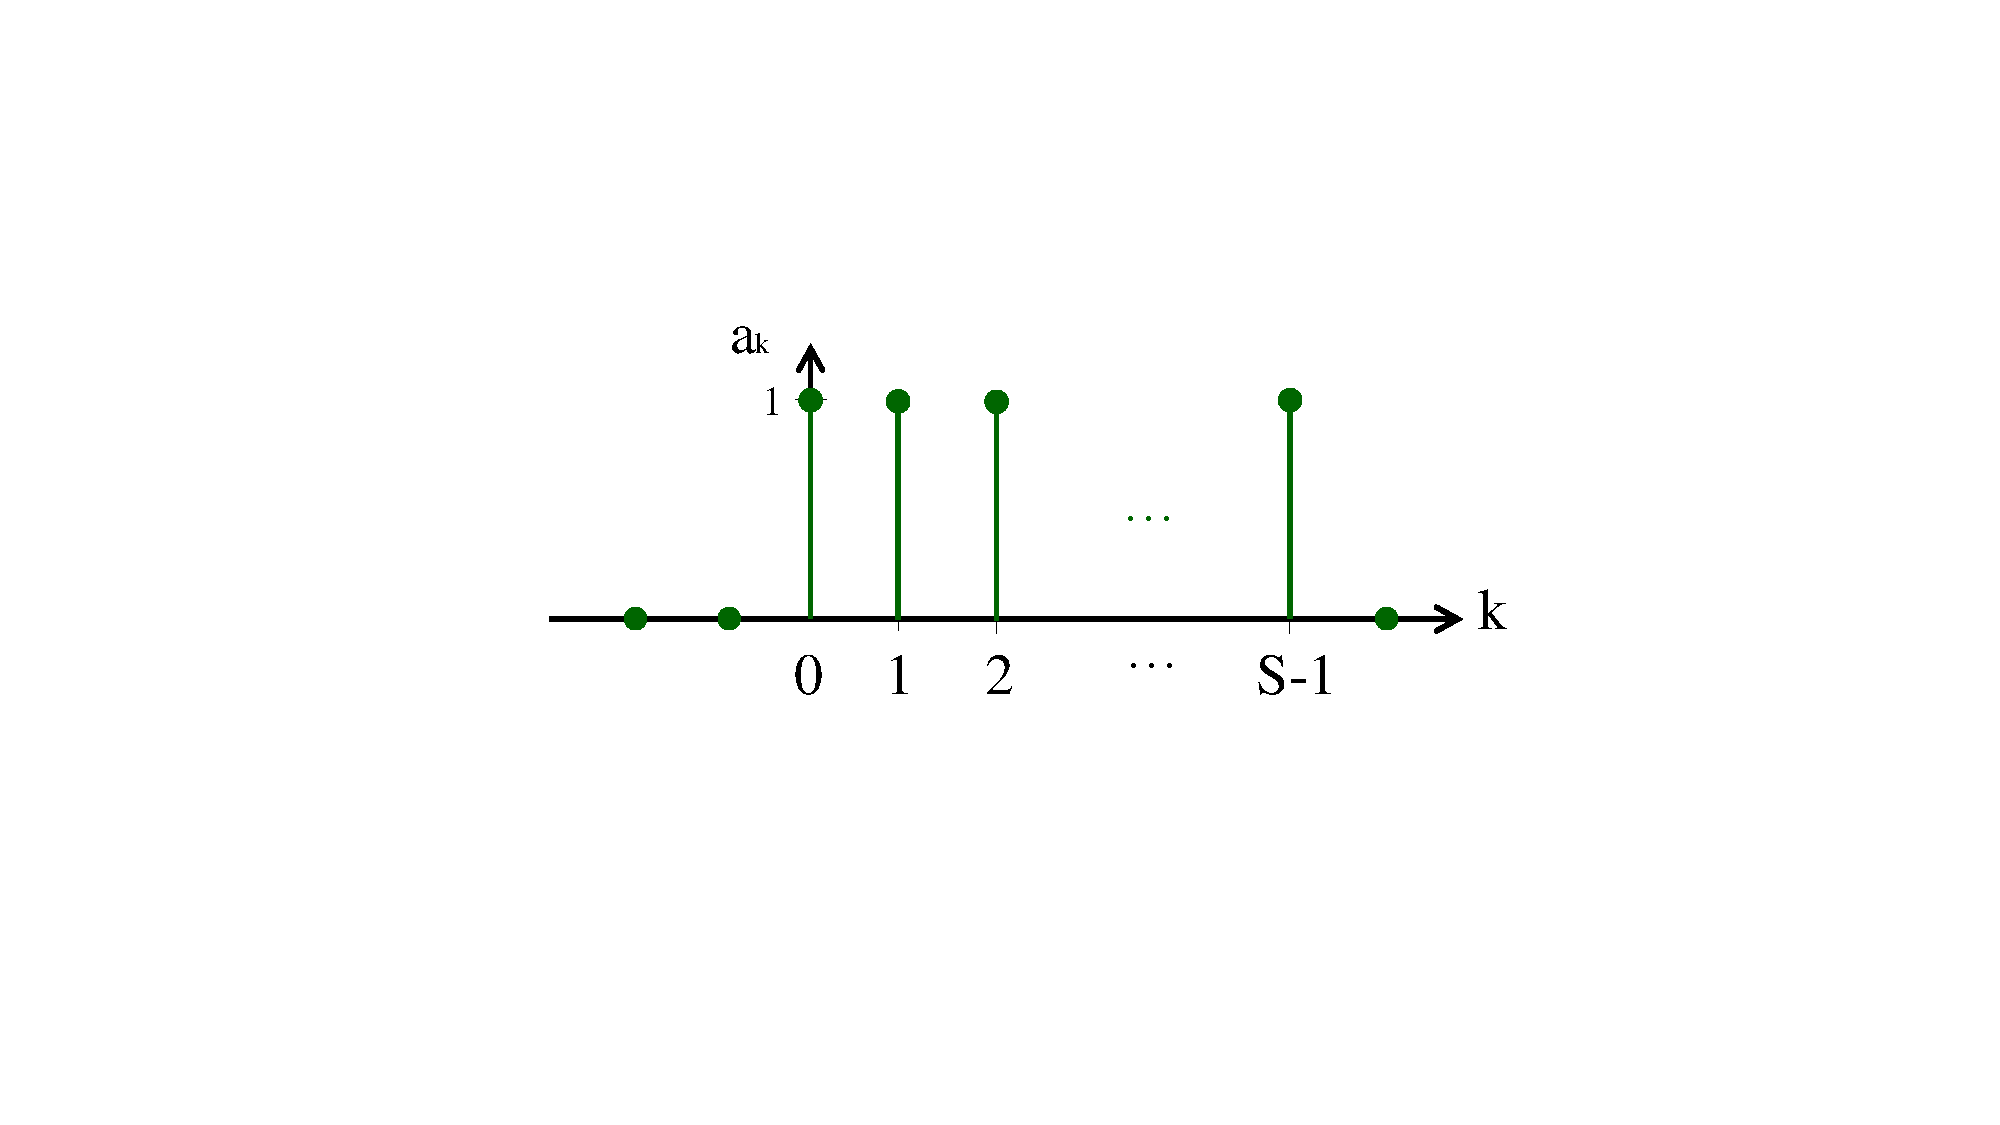
\includegraphics[trim =4cm 7cm 5cm 4cm, clip, width=0.70\textwidth]{graphics/SDP_square_window.pdf}
	\caption{Square window weighting}
	\label{fig:SDP_square_window}
\end{figure}
The weighting coefficients  $a_k$ can be chosen in different ways. One may be to do a square window weighting (see figure \ref{fig:SDP_square_window}), where in total $S$ previous values of $\vec{u}$ are taken into account and weighted equally (moving average). But usually it is better to weight the older values less than newer ones. Therefor an exponential weighting  is used commonly.\\
\mybox{
\textbf{Exponential weighting (Exponential Window):} $a_k=\eta^k;\quad |\eta|\leq 1$
}\\

\begin{doublespace}
$\ma{\hat{R}}[n]=\frac{\sum\limits_{k=0}^{\infty}\eta^k\vec{u}[n-k]\vec{u}^H[n-k]}{\underbrace{\sum\limits_{k=0}^{\infty}\eta^k}_{\frac{1}{1-\eta}}}$\\
To simplify the implementation of the calculation a recursive equation should be derived:\\
$\ma{\hat{R}}[n]=(1-\eta)\sum\limits_{k=0}^{\infty}\eta^k\vec{u}[n-k]\vec{u}^H[n-k]$\\
\begin{flalign*}
\ma{\hat{R}}[n+1]&=(1-\eta)\sum\limits_{k=0}^{\infty}\eta^k\vec{u}[n+1-k]\vec{u}^H[n+1-k]&&\\
&=(1-\eta)\sum\limits_{k+1=0}^{\infty}\eta^{k+1}\vec{u}[n-k]\vec{u}^H[n-k]&&\\
&=(1-\eta)\eta\sum\limits_{k=-1}^{\infty}\eta^{k}\vec{u}[n-k]\vec{u}^H[n-k]&&\\
&=\eta\underbrace{(1-\eta)\sum\limits_{k=0}^{\infty}\eta^{k}\vec{u}[n-k]\vec{u}^H[n-k]}_{\ma{\hat{R}}[n]} + (1-\eta)\underbrace{\eta\eta^{-1}}_{1}\vec{u}[n+1]\vec{u}^H[n+1]
\end{flalign*}
\mybox{
$\ma{\hat{R}}[n+1]=\eta\ma{\hat{R}}[n] + (1-\eta)\vec{u}[n+1]\vec{u}^H[n+1]$
}
$\vec{\hat{p}}[n+1]=\eta\vec{\hat{p}}[n](1-\eta)\vec{u}[n+1]d^*[n+1]$\\ \\
\mybox{
\textbf{SDP (Steepest Descent Procedure):}\\
\pfeil with optimal step size and estimation of correlation matrix and correlation vector\\
\pfeil procedure never stops. \\
\textbf{Input:} $\vec{u}[n],\quad d[n]$\\
\textbf{Output:} sequence of $\vec{w}[n]$\\
\begin{tabular}{ll}
	1. Init: &$\ma{\hat{R}}\leftarrow\ma{0},\quad\vec{\hat{p}}\leftarrow \vec{0},\quad \vec{w}\leftarrow \vec{0},\quad n\leftarrow0$\\
	2. Estimation: &$\ma{\hat{R}}\leftarrow\eta\ma{\hat{R}}+(1-\eta)\vec{u}[n+1]\vec{u}^H[n+1]$\\
	&$\vec{\hat{p}}\leftarrow \eta\vec{\hat{p}}[n](1-\eta)\vec{u}[n+1]d^*[n+1]$\\
  3. Weight update: &$\vec{\hat{r}}\leftarrow\vec{\hat{p}}-\ma{\hat{R}}\vec{w}$\\
	&$\hat{\mu}\leftarrow\frac{\vec{\hat{r}}^H\vec{\hat{r}}}{\vec{\hat{r}}H\ma{\hat{R}}\vec{\hat{r}}}$\\
	&$\vec{w}\leftarrow\vec{w}\hat{\mu}\vec{\hat{r}}$\\
	4. Output \vec{w} for $\vec{w}[n+1]$&\\
	5. $n\leftarrow n+1$, go to step 2&\\
\end{tabular}}\\
\textbf{Note:} This is called procedure and not algorithm since an algorithm needs to stop (finish) after a finite time (by definition). That's not the case here.\\
\begin{figure}[H]
	\centering
		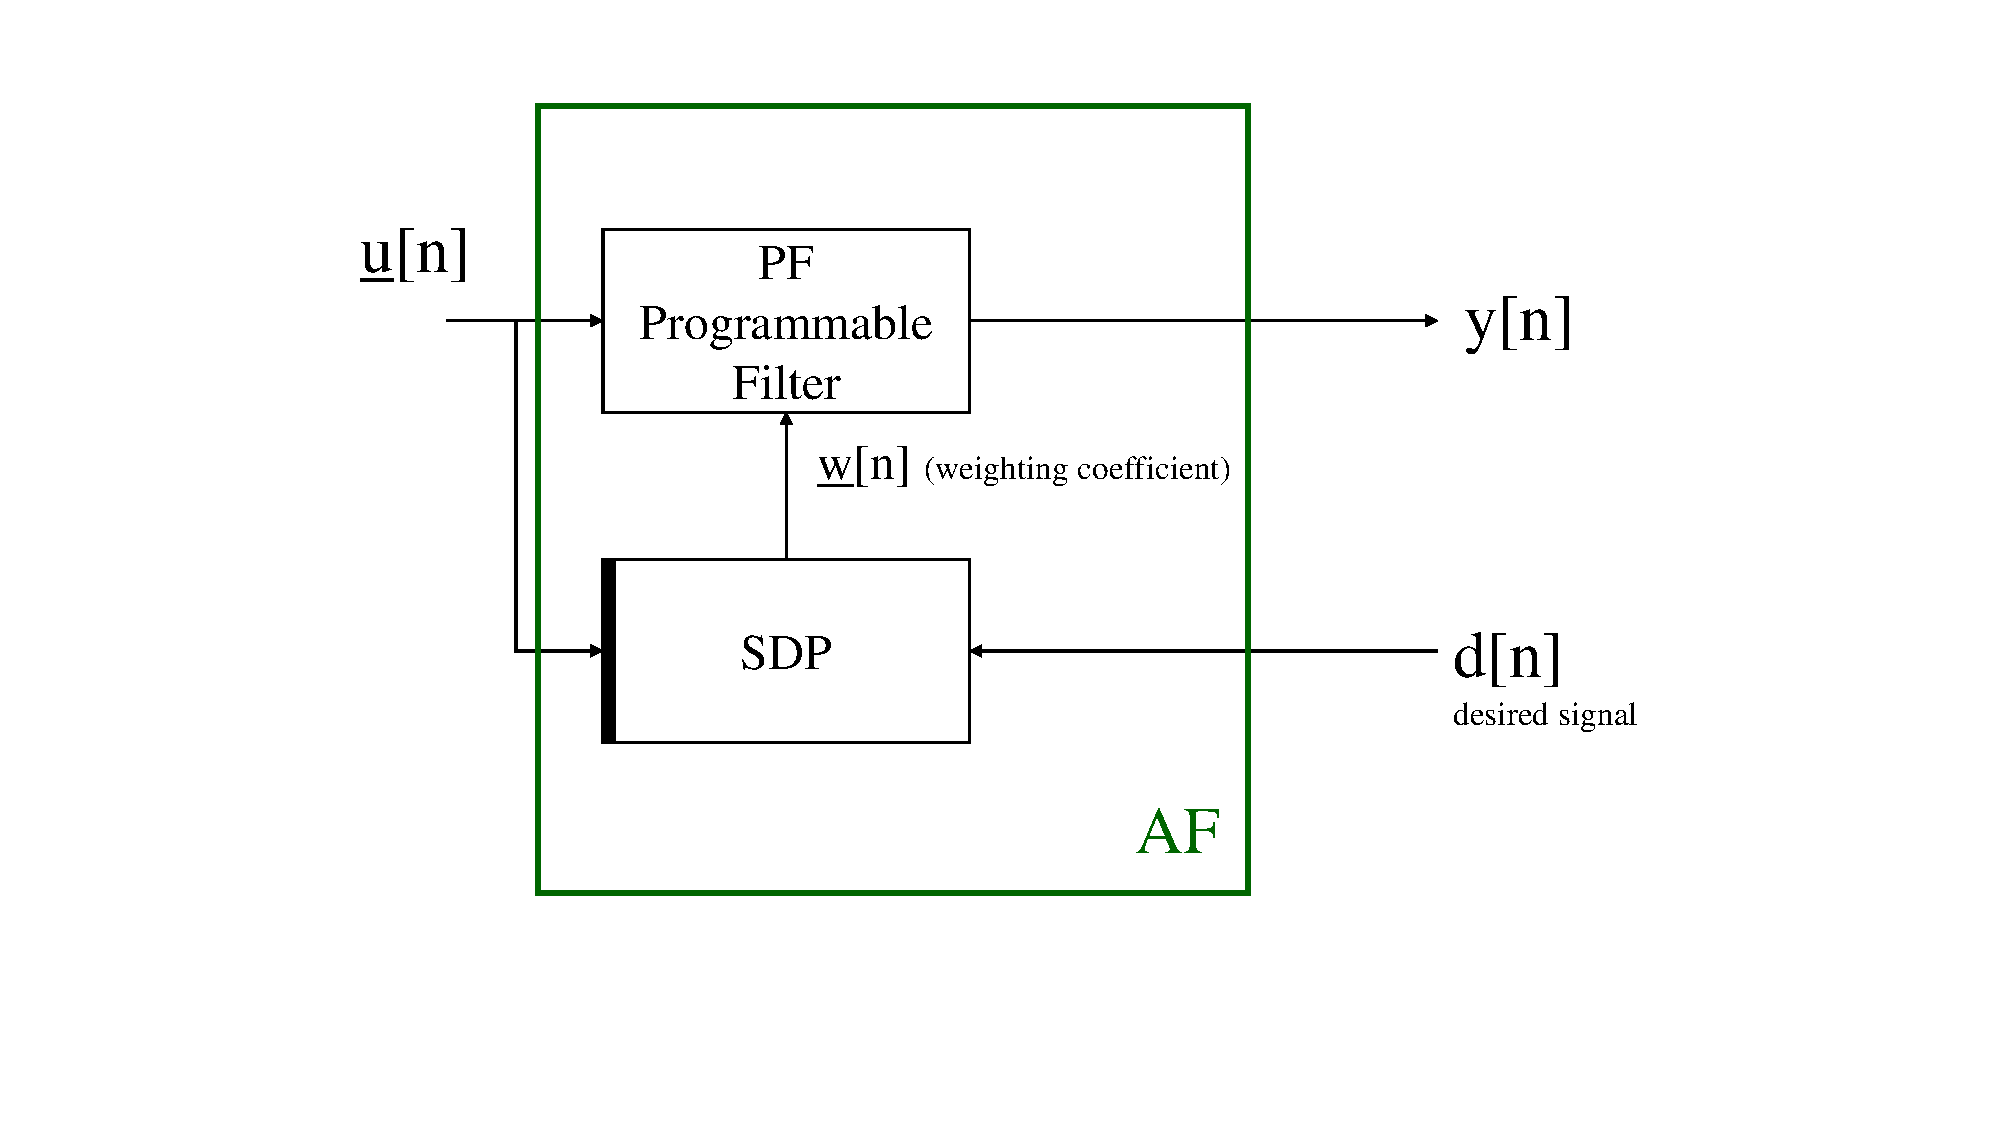
\includegraphics[trim =4cm 3cm 4cm 1cm, clip, width=0.70\textwidth]{graphics/adaptive_filter_with_SDP.pdf}
	\caption{Block diagram of an adaptive filter (AF) using the ``Steepest Descent Procedure''}
	\label{fig:adaptive_filter_with_SDP}
\end{figure}

\begin{tabular}{ll}
\textbf{Note:}&$\eta$ close to 0:\\
&$\quad$ Pro: Track fast changing channels better\\
&$\quad$ Con: Poor estimation for slow changing channels\\
&\\
&$\eta$ close to 1:\\
&$\quad$ Pro: Good estimation for slow changing channels\\
&$\quad$ Con: Bad tracking of fast changing channels\\
&\\
\end{tabular}

\textbf{Note: LMS-Procedure:}\\
$\text{``LMS''}=\lim\limits_{\eta\rightarrow 0}\text{``SDP''}$\\
$\ma{\hat{R}}[n+1]=\vec{u}[n]\vec{u}^H[n], \quad \vec{\hat{p}}[n]=\vec{u}[n]d^*[n]$\\
$\vec{w}[n+1]=\vec{w}[n]+\mu\vec{u}[n]\vec{e}^*[n]$\\
$\vec{e}[n]=d[n]-\vec{w}^H[n]\vec{u}[n]$\\
$\mu=\frac{1}{||\vec{u}[n]||_2^2+a};\qquad a>0$\\
or $\mu=\const$\\
\rule{\textwidth}{0.4pt}

\textbf{Application: linearly constraint minimum variance problem}

$y[n]=\vec{w}^H\vec{u}[n]$\\
$\min \underbrace{E[|y[n]|^2]}_{\vec{w}^H \underbrace{E[\vec{u}[n]\vec{u}^H[n]]}_{\ma{R}=\ma{A}}\vec{w}}, \text{ s. t. } \ma{B}\vec{w}=\vec{c}$\\
$\vec{w}=\vec{w}_q-\ma{V}_2\vec{w}_a$\\
$y[n]=\vec{w}_q^H\vec{u}[n]-\vec{w}_a^H\ma{V}_2\vec{u}[n]$\\

\begin{figure}[H]
	\centering
		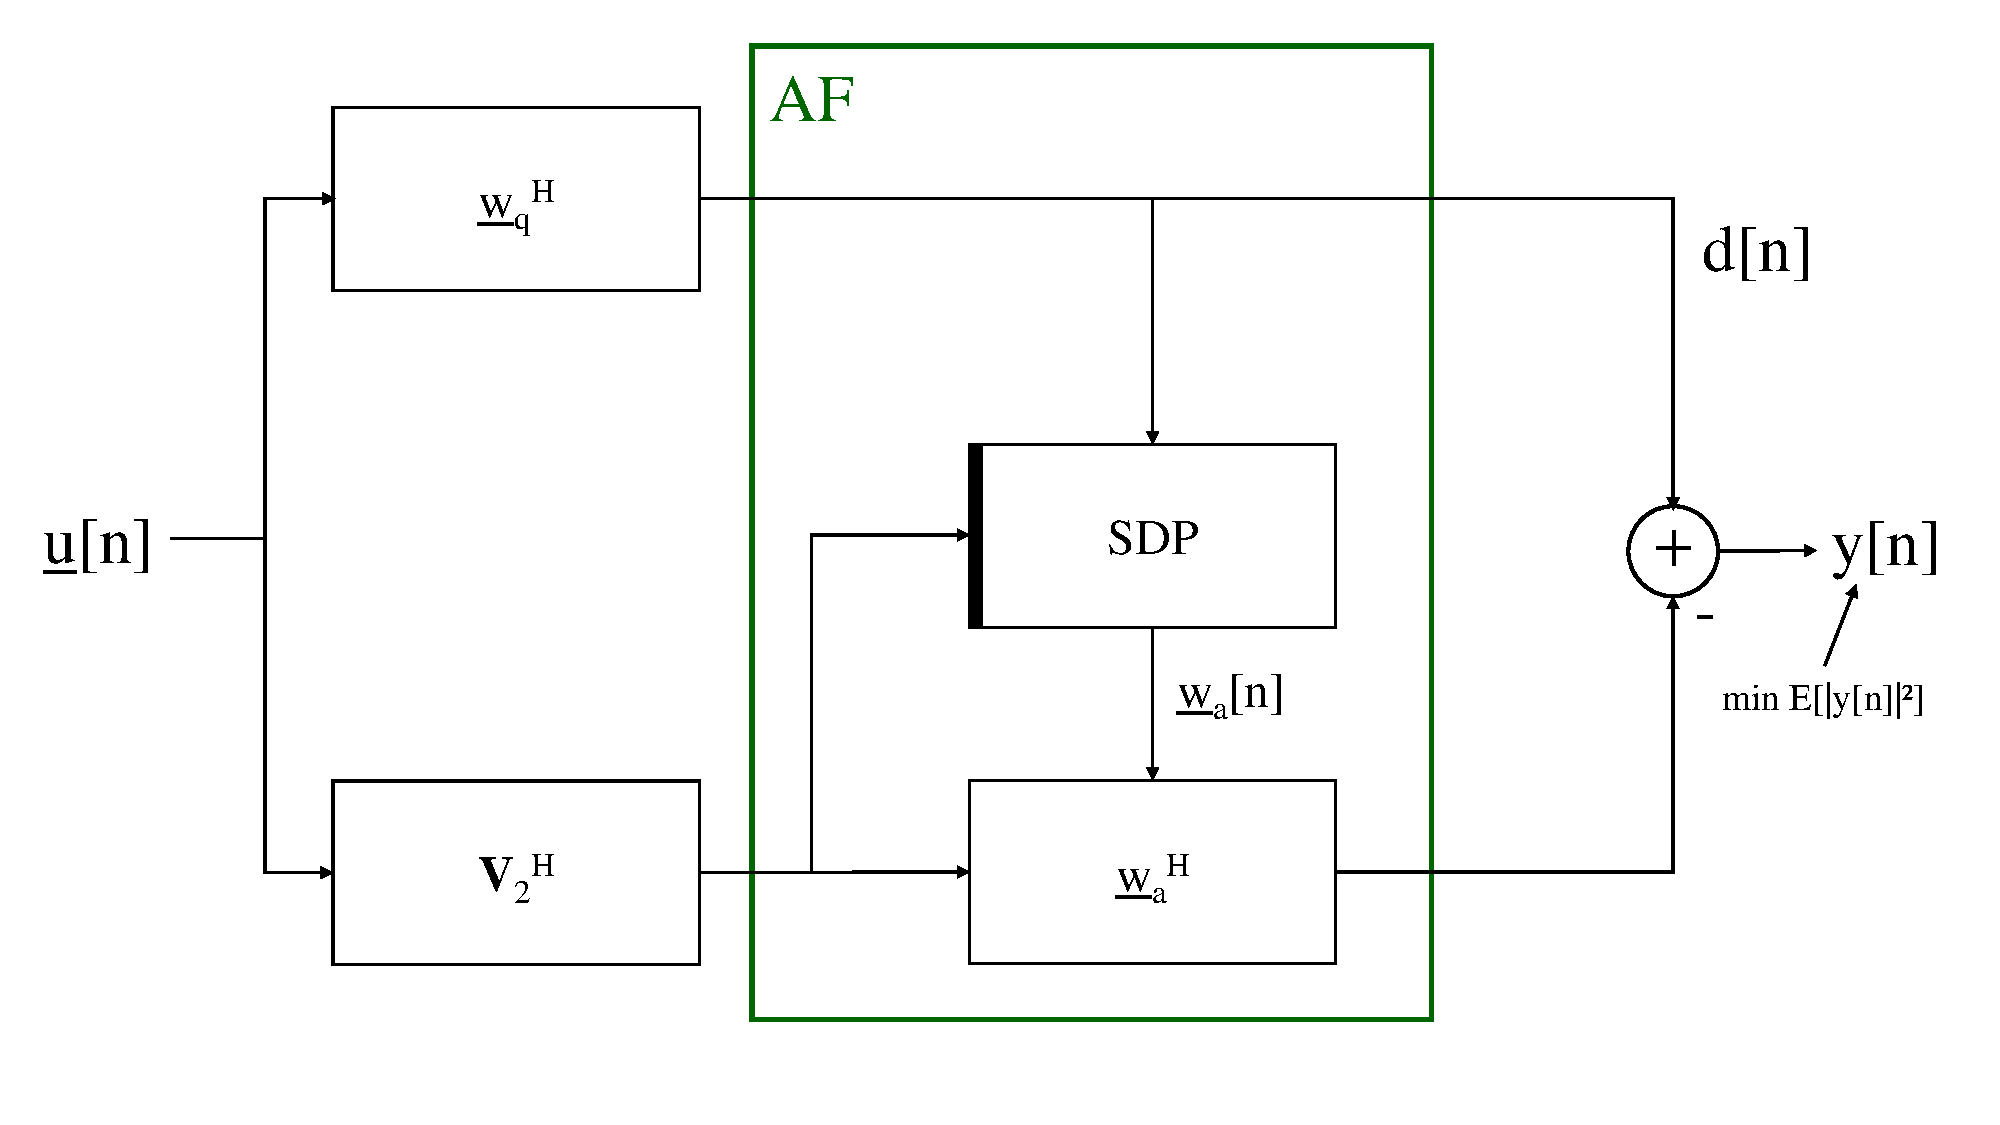
\includegraphics[trim =0cm 1.5cm 1cm 0cm, clip, width=1.00\textwidth]{graphics/Linearly_constraint_minimum_variance_problem.pdf}
	\caption{Linearly constraint minimum variance problem}
	\label{fig:Linearly_constraint_minimum_variance_problem}
\end{figure}
\end{doublespace}

\subsubsection{Example: Digital Spectrum Analyser (linear)}\label{sssec:dsa}
\begin{doublespace}
$u[n]=\sum\limits_{k=1}^{d}s_k \cdot e^{j2\pi f_k T n}+\nu[n]$\\
With following variables:\\
\begin{tabular}{rl}
$d$:& number of complex sinusoids\\
$f_1,\,f_2\,\ldots\,f_d$:& frequencies\\
$|s_1|,\,|s_2|\,\ldots\,|s_d|$:&amplitudes\\
$\arg S_1,\,\arg S_2,\,\ldots\,\arg S_d$:& phase\\
$T$:& sampling time\\
$\nu[n]$:& noise\\
\end{tabular}
 
We want to know: $d,\,f_1,\,f_2,\,\ldots\,f_d,\,|s_1|,\,|s_2|\,\ldots\,|s_d|$\\
\begin{flalign*}
\vec{u}[n]&=\mat{u[n]\\u[n-1]\\\svdots\\u[n-(M-1)]}=\mat{\sum\limits_{k=1}^{d}s_k \cdot e^{j2\pi f_k T\cdot n}+\nu[n]\\\sum\limits_{k=1}^{d}s_k \cdot e^{j2\pi f_k T \cdot (n-1)}+\nu[n-1]\\\svdots\\\sum\limits_{k=1}^{d}s_k \cdot e^{j2\pi f_k T\cdot (n-(M-1))}+\nu[n-(M-1)]}&&\\
&=\sum\limits_{k=1}^{d}s_k\underbrace{\mat{1\\e^{-j2\pi f_k T}\\\svdots\\e^{-(M-1)j2\pi f_k T}}}_{\vec{a}(f_k)}e^{j2\pi f_k T\cdot n}+\mat{\nu[n]\\\nu[n-1]\\\svdots\\\nu[n-(M-1)]}
\end{flalign*}
\mybox{
$\vec{u}[n]=\sum\limits_{k=1}^{d}s_k\vec{a}(f_k)e^{j2\pi f_k T n}+\vec{\nu}[n]$\\
}

\begin{figure}[H]
	\centering
		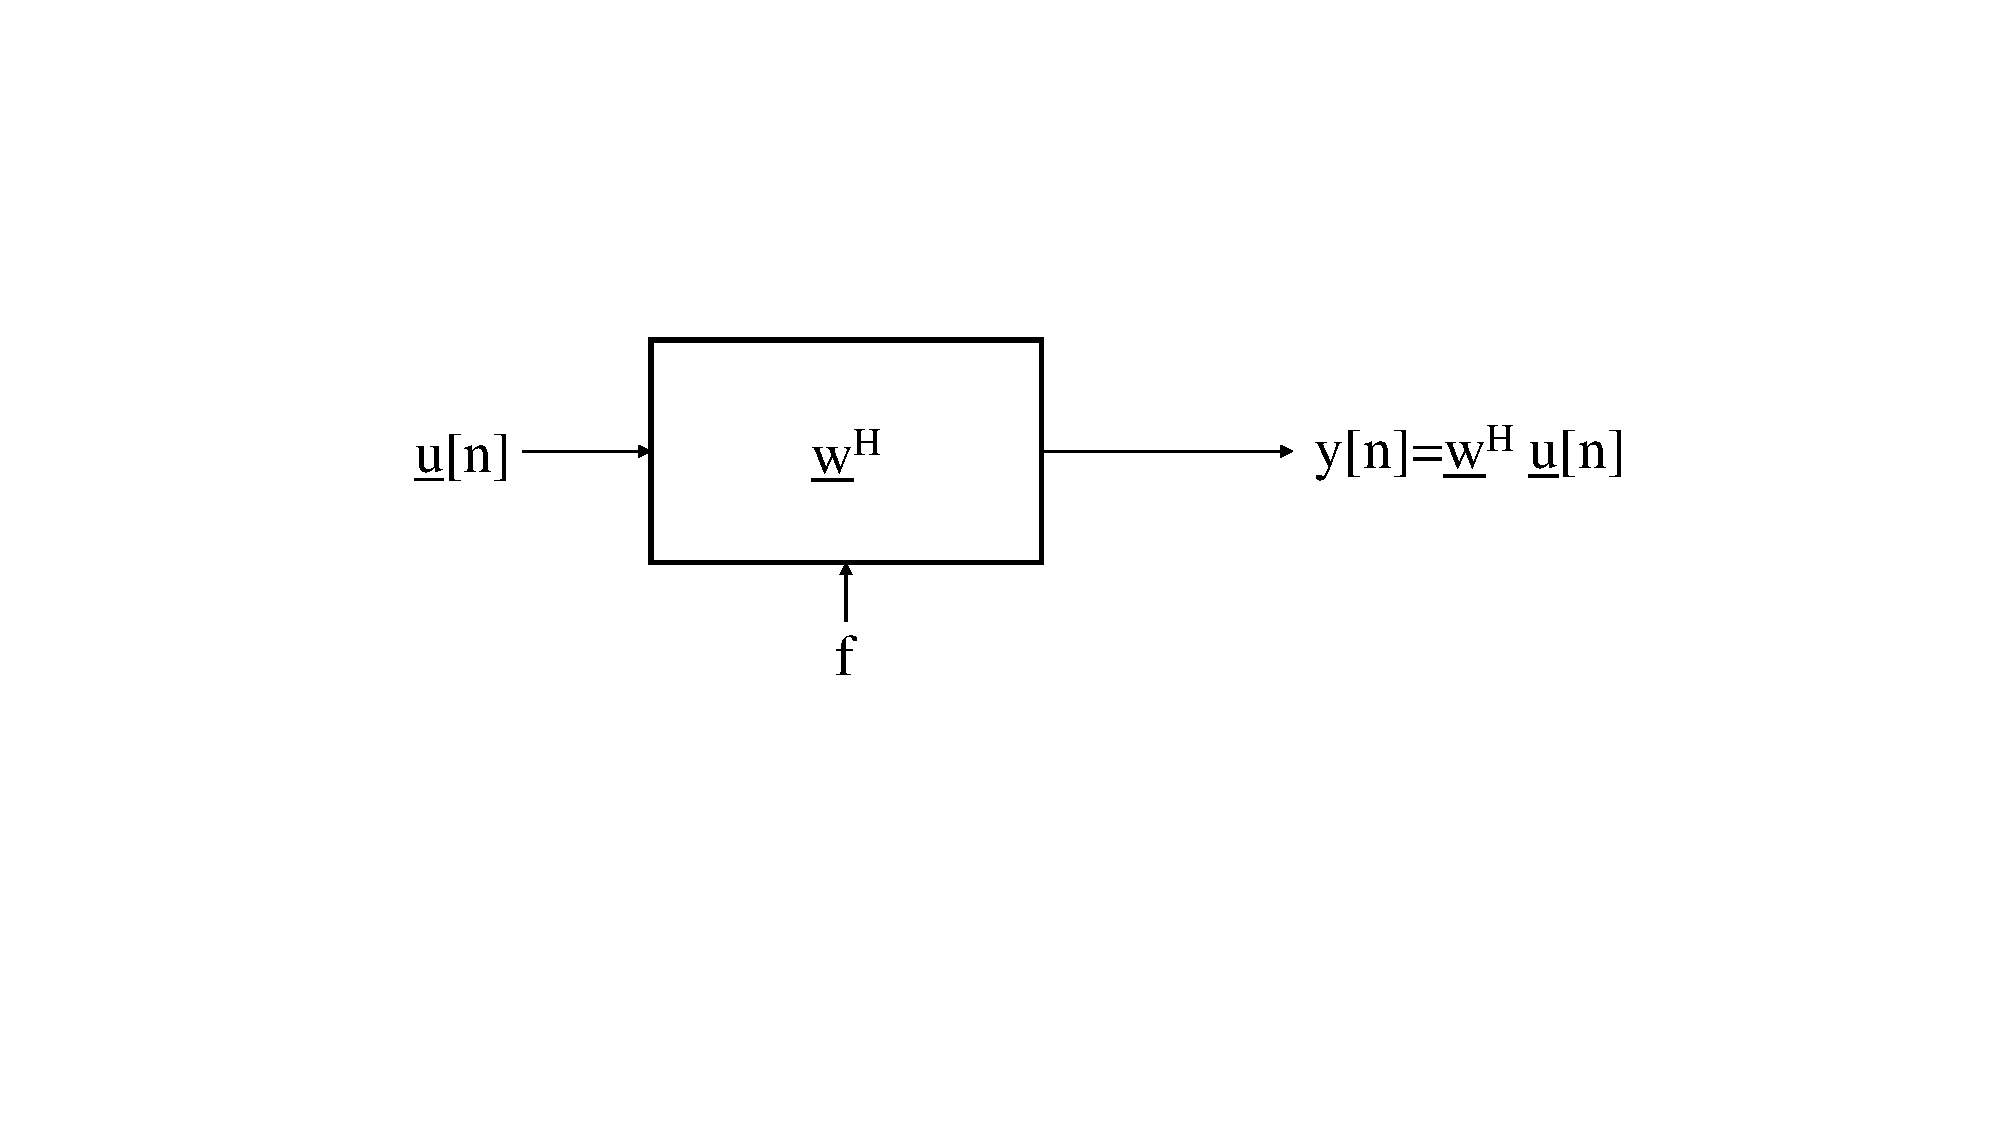
\includegraphics[trim =3cm 7cm 3cm 3cm, clip, width=0.70\textwidth]{graphics/ex_spectrum_analyzer.pdf}
	\caption{Block diagram of a Digital Spectrum Analyzer}
	\label{fig:ex_spectrum_analyzer}
\end{figure}

\begin{enumerate}
	\item $\vec{w}^H\vec{a}(f)=1\qquad \text{or } \underbrace{\vec{a}^H(f)}_{\ma{B}}\vec{w}=1$
	\item $\min \underbrace{E[|y[n]|^2]}_{\vec{w}^H\underbrace{E[\vec{u}[n]\vec{u}^H[n]]}_{\ma{A}}\vec{w}}$
\end{enumerate}
$\mathcal{L}=\vec{w}^H\ma{A}\vec{w}+\lambda(\vec{a}^H(f)\vec{w}-1)+(\vec{w}^H\vec{a}(f)-1)\lambda^*$\\
\mybox{
$\vec{w}_{opt}=\frac{\ma{A}^{-1}\vec{a}(f)}{\vec{a}^H(f)\ma{A}^{-1}\vec{a}(f)}$
}\\
$E[|y[n]|^2]=\vec{w}_{opt}^H\ma{A}\vec{w}_{opt}=\frac{1}{\vec{a}^H(f)\ma{A}^{-1}\vec{a}(f)}$\\ \ \\

$d=2,\quad M=3,\quad \sigma_\nu^2=0.001$\\
$S_1=1+j,\quad S_2=-1+2j,\quad T=0.25\,\mu\text{S}$\\
$|S_1|^2=2,\quad |S_2|^2=5$\\
$f_1=1\,\text{MHz},\quad f_2=1.7\,\text{MHz}$\\
Parameter: $\vec{a}(f_1)=\mat{1\\e^{-j2\pi f_1 T}\\e^{-j4\pi f_1 T}}\qquad \vec{a}(f_2)=\mat{1\\e^{-j2\pi f_2 T}\\e^{-j4\pi f_2 T}}$\\
Variable:\quad $\vec{a}(f)=\mat{1\\e^{-j2\pi f T}\\e^{-j4\pi f T}}$\\

\begin{flalign*}
\ma{A}&=E[\vec{u}[n]\vec{u}^H[n]]&&\\
&=|S_1|^2\vec{a}_1\vec{a}_1^H+|S_2|^2\vec{a}_2\vec{a}_2^H+0.001\ma{I}+S_1S_2^*e^{j2\pi(f_1-f_2)T n}+S_1^*S_2e^{-j2\pi(f_1-f_2)T n}
\end{flalign*}
$\ma{A}\leftarrow \underbrace{\ma{\bar{A}}}_{\text{time average}}=|S_1|^2\vec{a}_1\vec{a}_1^H+|S_2|^2\vec{a}_2\vec{a}_2^H+0.001\ma{I}$\\
$A_{11}=A_{22}=A_{33}=7.001$\\
$A_{21}=A_{32}=A_{12}^*=A_{23}^*=-4.455-j\,4.27$\\
$A_{31}=A_{13}^*=0.9389+j\,4.0451$\\


\begin{align*}
\ma{A}=&E[\vec{u}[n]\vec{u}^H[n]]=E\left[\left(\sum\limits_{k=1}^{2}s_k\vec{a}(f_k)e^{j2\pi f_k T n}+\vec{\nu}[n]\right)\left(\sum\limits_{k=1}^{2}s_k\vec{a}(f_k)e^{j2\pi f_k T n}+\vec{\nu}[n]\right)^H\right]\\
=&E\left[\left(s_1\vec{a}(f_1)e^{j2\pi f_1 T n}+s_2\vec{a}(f_2)e^{j2\pi f_2 T n}+\vec{\nu}[n]\right)
\left(s_1^*\vec{a}(f_1)^He^{-j2\pi f_1 T n}+s_2^*\vec{a}(f_2)^He^{-j2\pi f_2 T n}+\vec{\nu}[n]^H\right)\right]\\
=&\abs{s_1}\vec{a}_1\vec{a}_1^H+\abs{s_2}\vec{a}_2\vec{a}_2^H+\sigma_\nu^2\ma{I}+s_1s_2^*\vec{a}(f_1)\vec{a}(f_2)^He^{j2\pi (f_1-f_2) T n}+
s_2s_1^*\vec{a}(f_2)\vec{a}(f_1)^He^{j2\pi (f_2-f_1) T n}
\end{align*}

$\ma{\bar{A}}=\mat{7.001&-4.455+\j 4.27&0.9389-\j 4.0451\\-4.455-\j 4.27&7.001&-4.455+\j 4.27\\ 0.9389+\j 4.0451 & -4.455-\j 4.27 & 7.001}$

$\ma{\bar{A}}^{-1}=100\cdot\mat{2.0858&1.8569-\j 3.0297&-0.9460-\j 1.8553\\1.8569+\j 3.0297&6.0603&1.8569-\j 3.0297\\ -0.9460+\j 1.8553 & 1.8569+\j 3.0297 & 2.0858}$

\begin{figure}[H]
	\centering
		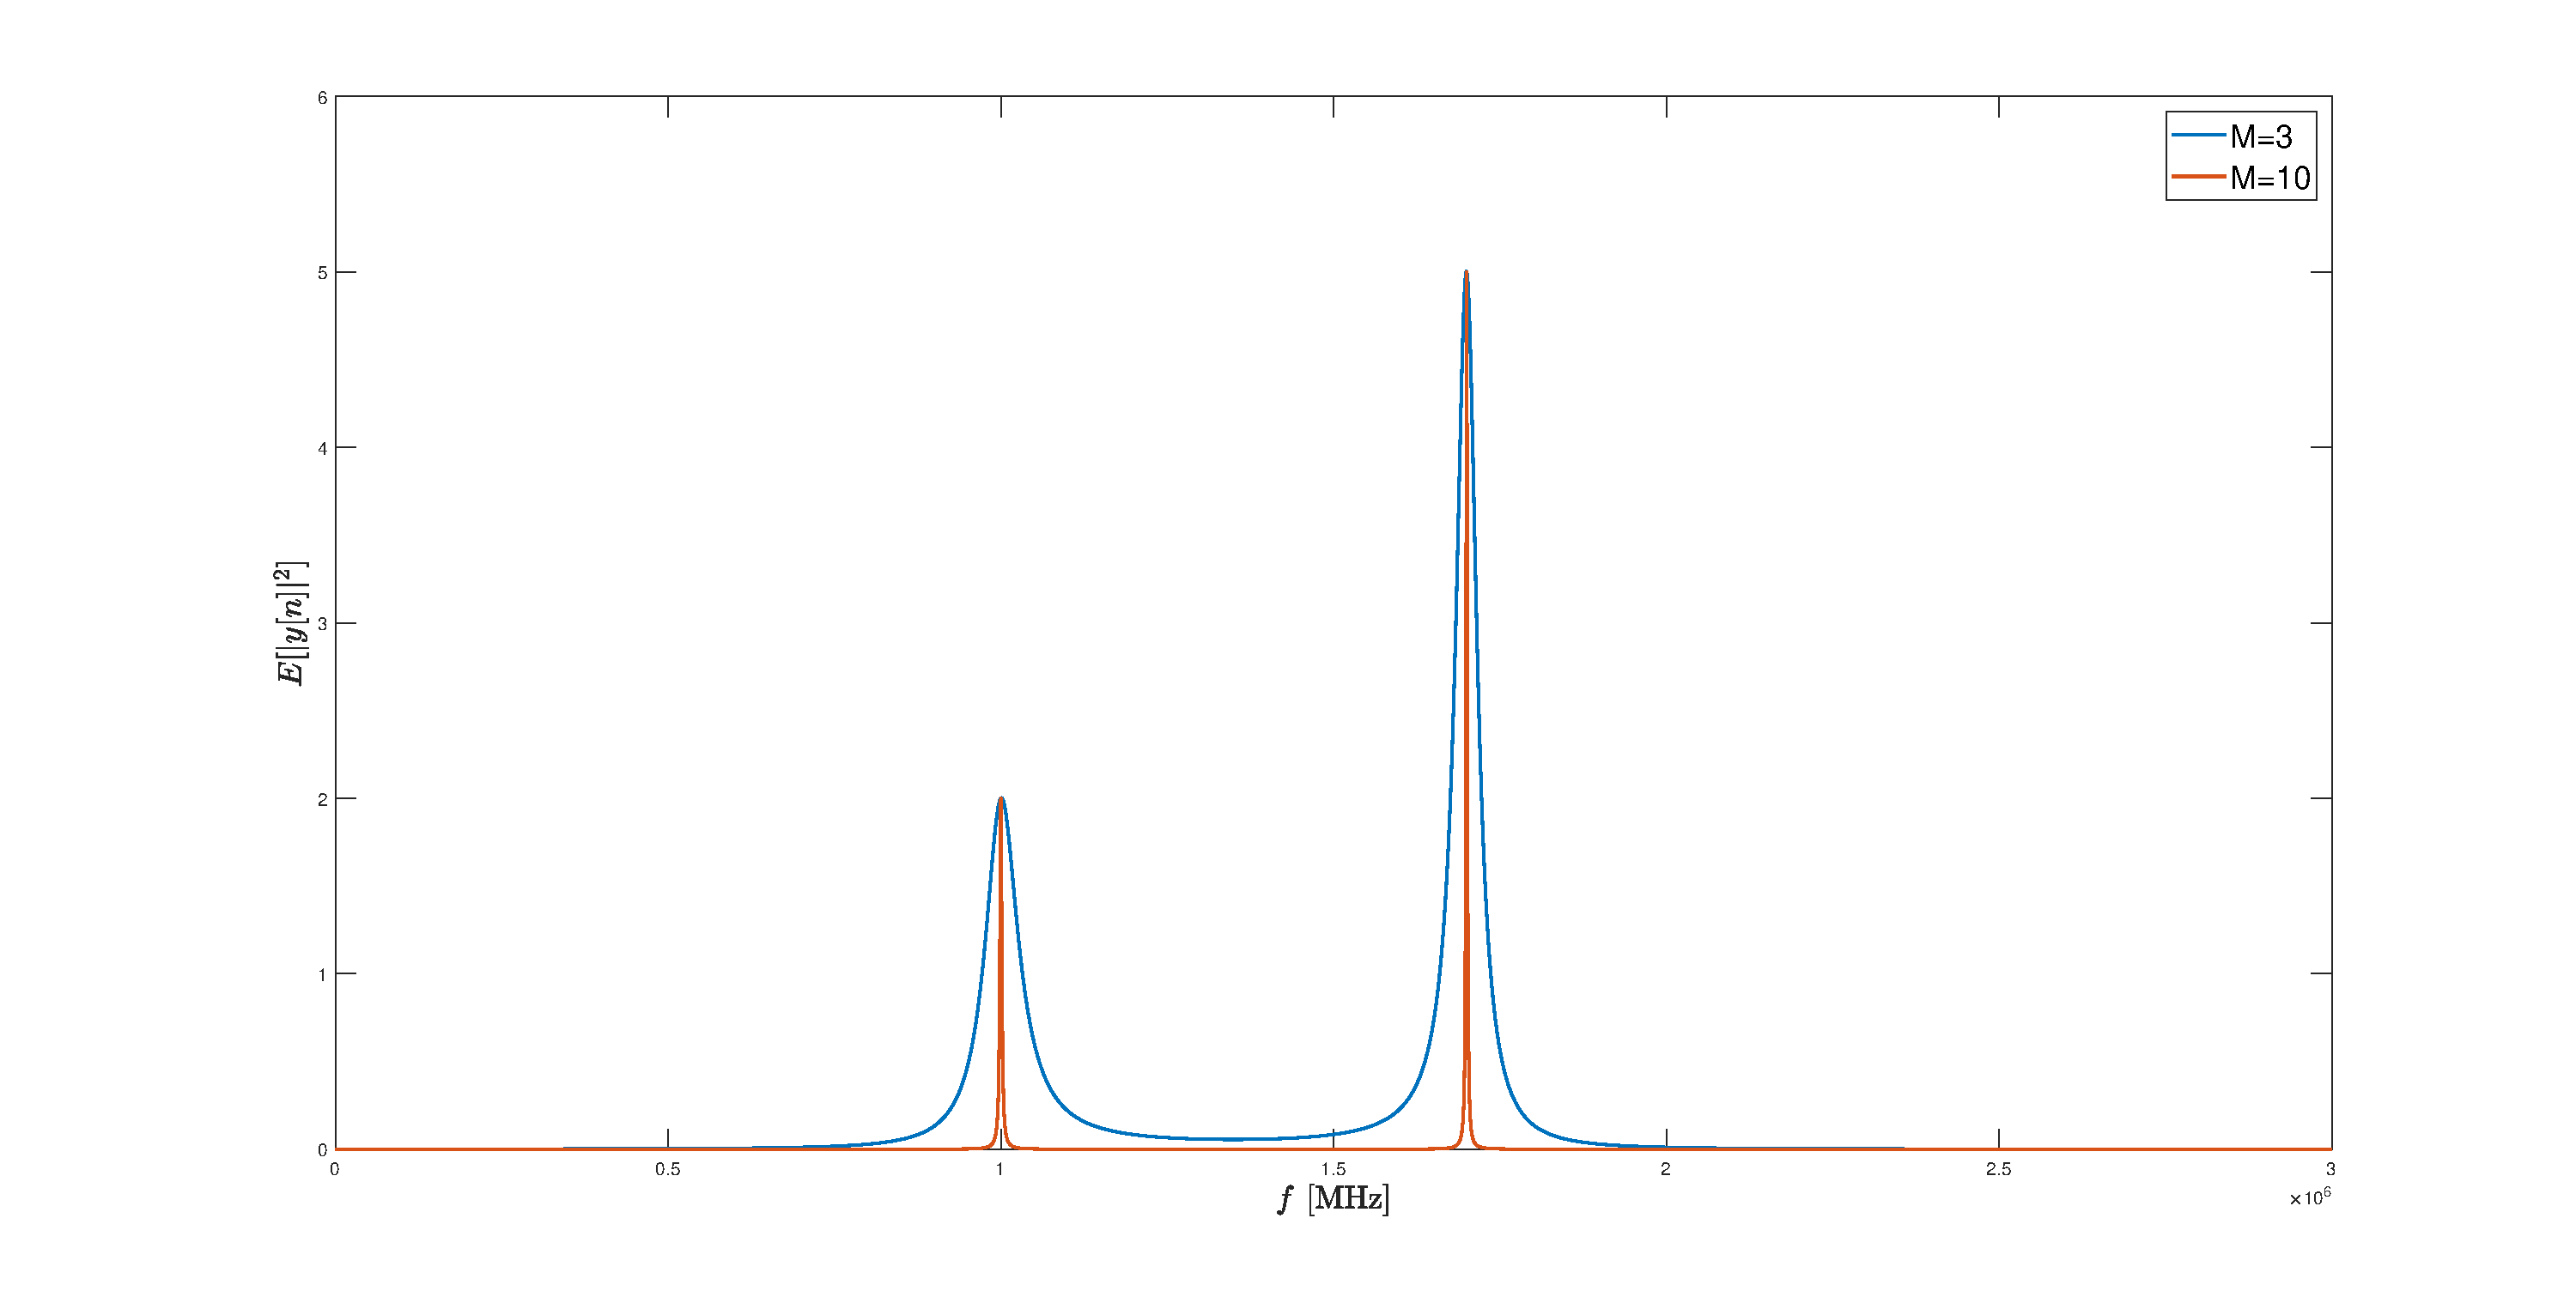
\includegraphics[trim =4cm 1cm 4cm 1cm, clip, width=1.00\textwidth]{graphics/ex_spectrum_analyzer_result_plot.pdf}
	\caption{Plot of the result for two difference memory depth ($M=3$ and $M=10$)}
	\label{fig:ex_spectrum_analyzer_result_plot}
\end{figure}

\end{doublespace}

